%========================================
% MatinBook - Advanced Algorithms & Mathematics
% Chapter 1: Asymptotic Analysis and Complexity
%========================================

\makeatletter
\def\input@path{{../}}
\makeatother

\documentclass{matinbook}

\addbibresource{../references.bib}

\title{الگوریتم‌های پیشرفته و مبانی ریاضی}
\author{تیم توسعه MatinBook}
\date{تابستان ۱۴۰۵}

\begin{document}
    
    %========================================
    % COVER
    %========================================
    \makecover
    {الگوریتم‌های پیشرفته\\و مبانی ریاضی}
    {از نظریه تا پیاده‌سازی}
    {تیم توسعه MatinBook}
    {تابستان ۱۴۰۵}
    
    \makebackcover{%
        \textbf{الگوریتم‌های پیشرفته و مبانی ریاضی}
        کتابی جامع برای دانشجویان تحصیلات تکمیلی
        و علاقه‌مندان به علوم کامپیوتر نظری است.
        
        \textbf{در این کتاب می‌آموزید:}
        \begin{itemize}
            \item تحلیل مجانبی و پیچیدگی الگوریتم‌ها
            \item راهبردهای طراحی الگوریتم (تقسیم و حل، پویا، حریصانه)
            \item الگوریتم‌های گراف پیشرفته و شار بیشینه
            \item الگوریتم‌های تصادفی و کاربردهای آن
            \item ساختمان داده‌های پیشرفته (AVL، B-Tree، هیپ فیبوناچی)
            \item نظریه اعداد محاسباتی و رمزنگاری
            \item جبر خطی عددی و بهینه‌سازی محدب
        \end{itemize}
        
        \textbf{ویژگی‌های کتاب:}
        \begin{itemize}
            \item اثبات‌های دقیق ریاضی برای تمام قضایا
            \item پیاده‌سازی الگوریتم‌ها به زبان Python و C++
            \item بیش از ۱۰۰ تمرین با پاسخ تشریحی
            \item نمودارها و تصاویر آموزشی
        \end{itemize}
        
        \textbf{ساخته شده با MatinBook نسخه ۱}
    }
    
    %========================================
    % TITLE PAGE
    %========================================
    \maketitle
    
 
    
    %========================================
    % COPYRIGHT
    %========================================
    \thispagestyle{empty}
    \vspace*{5cm}
    \begin{center}
        {\large\textbf{حقوق نشر}}\\[1cm]
        \textbf{الگوریتم‌های پیشرفته و مبانی ریاضی}\\[0.5cm]
        نسخه ۱.۰ --- تابستان ۱۴۰۵\\[1cm]
        \lr{Copyright \copyright\ 2026 MatinBook Project}\\
        \lr{Licensed under MIT License}
    \end{center}
    \clearpage
    \frontmatter
    
    %========================================
    % PREFACE
    %========================================
    \chapter*{پیشگفتار}
    \addcontentsline{toc}{chapter}{پیشگفتار}
    
    این کتاب برای دانشجویان تحصیلات تکمیلی علوم کامپیوتر،
    ریاضیات کاربردی و مهندسی نرم‌افزار نوشته شده است.
    هدف ما ارائه تلفیقی از نظریه و عمل است: از یک سو،
    اثبات‌های دقیق ریاضی برای درک عمیق مفاهیم،
    و از سوی دیگر، پیاده‌سازی‌های واقعی به زبان‌های
    Python و C++ برای تسلط عملی.
    
    \section*{پیش‌نیازها}
    
    \begin{itemize}
        \item آشنایی با ساختمان داده‌های پایه (آرایه، لیست، درخت، گراف)
        \item دانش برنامه‌نویسی به یک زبان اصلی
        \item ریاضیات عمومی (حد، مشتق، انتگرال، جبر خطی مقدماتی)
        \item مبانی نظریه گراف و ترکیبیات
    \end{itemize}
    
    \clearpage
    
    %========================================
    % TABLE OF CONTENTS
    %========================================
    \tableofcontents
    \clearpage
    \mainmatter
    
    
        \listoffigures
    \clearpage
    
    \listoftables
    \clearpage
    
    \listofalgorithms
    \clearpage
    
    %========================================
    % CHAPTER 1: Asymptotic Analysis
    %========================================
    \chapter{تحلیل مجانبی و پیچیدگی الگوریتم‌ها}
    \label{chap:asymptotic}
    
    \section{مقدمه}
    
    تحلیل الگوریتم\index{تحلیل الگوریتم} قلب علوم کامپیوتر نظری است.
    پیش از آنکه الگوریتمی را پیاده‌سازی کنیم، باید بدانیم
    با افزایش اندازه ورودی، زمان اجرا و حافظه مصرفی
    چگونه رشد می‌کنند. این تحلیل به ما کمک می‌کند
    الگوریتم مناسب را برای هر مسئله انتخاب کنیم.
    
    \begin{definition}[تحلیل الگوریتم]
        تحلیل الگوریتم فرایند پیش‌بینی \textbf{نرخ رشد}
        منابع مصرفی (زمان، حافظه) بر حسب \textbf{اندازه ورودی}
        است، بدون وابستگی به سخت‌افزار یا زبان برنامه‌نویسی خاص.
        \label{def:algorithm-analysis}
    \end{definition}
    
    \section{نمادهای مجانبی}
    
    سه نماد اصلی برای توصیف رفتار مجانبی توابع
    وجود دارد که توسط دانلد کنوث\index{کنوث، دانلد}
    معرفی شده‌اند \cite{knuth1984}.
    
    \subsection{کران بالا: نماد $O$ بزرگ}
    
    \begin{definition}[$O$-بزرگ]
        تابع $f(n)$ از مرتبه $O(g(n))$ است،
        و می‌نویسیم $f(n) = O(g(n))$، اگر اعداد ثابت
        مثبت $c$ و $n_{0}$ وجود داشته باشند
        به طوری که برای تمام $n \geq n_{0}$:
        \[
        0 \leq f(n) \leq c \cdot g(n)
        \]
        \label{def:big-o}
    \end{definition}
    
    به عبارت دیگر، $g(n)$ یک \textbf{کران بالای مجانبی}
    برای $f(n)$ است. $f(n)$ \textbf{سریع‌تر} از
    $c \cdot g(n)$ رشد نمی‌کند.
    
    \begin{example}[اثبات $O$-بزرگ]
        ثابت کنید $f(n) = 3n^{2} + 5n + 2$ از مرتبه $O(n^{2})$ است.
        
        \textbf{راه حل:}
        برای $n \geq 1$ داریم:
        \begin{align*}
            3n^{2} + 5n + 2 &\leq 3n^{2} + 5n^{2} + 2n^{2} \\
            &= 10n^{2}
        \end{align*}
        بنابراین با $c = 10$ و $n_{0} = 1$،
        شرط برقرار است.
        \label{ex:big-o-proof}
    \end{example}
    
    \subsection{کران پایین: نماد Ω بزرگ}
    
    \begin{definition}[$\Omega$-بزرگ]
        تابع $f(n)$ از مرتبه $\Omega(g(n))$ است اگر
        اعداد ثابت مثبت $c$ و $n_{0}$ وجود داشته باشند
        به طوری که برای تمام $n \geq n_{0}$:
        \[
        0 \leq c \cdot g(n) \leq f(n)
        \]
        \label{def:big-omega}
    \end{definition}
    
    $\Omega$ یک \textbf{کران پایین مجانبی} ارائه می‌دهد.
    $f(n)$ \textbf{حداقل} به سرعت $c \cdot g(n)$ رشد می‌کند.
    
    \begin{example}[اثبات $\Omega$-بزرگ]
        ثابت کنید $f(n) = 3n^{2} + 5n + 2$ از مرتبه $\Omega(n^{2})$ است.
        
        \textbf{راه حل:}
        برای $n \geq 1$:
        \begin{align*}
            3n^{2} + 5n + 2 &\geq 3n^{2}
        \end{align*}
        بنابراین با $c = 3$ و $n_{0} = 1$،
        شرط برقرار است.
        \label{ex:omega-proof}
    \end{example}
    
    \subsection{کران بالا: نماد O بزرگ}
    
    \begin{definition}[$\Theta$]
        $f(n) = \Theta(g(n))$ اگر و تنها اگر
        $f(n) = O(g(n))$ و $f(n) = \Omega(g(n))$.
        \label{def:theta}
    \end{definition}
    
    $\Theta$ یک \textbf{کران مجانبی دقیق} است:
    $f(n)$ و $g(n)$ با نرخ یکسانی رشد می‌کنند.
    
    \begin{theorem}[شرط $\Theta$]
        $f(n) = \Theta(g(n))$ اگر و تنها اگر
        اعداد ثابت $c_{1}, c_{2} > 0$ و $n_{0}$ وجود داشته باشند
        که برای $n \geq n_{0}$:
        \[
        0 \leq c_{1} \cdot g(n) \leq f(n) \leq c_{2} \cdot g(n)
        \]
        \label{thm:theta-condition}
    \end{theorem}
    
    \section{تحلیل الگوریتم‌های بازگشتی}
    
    بسیاری از الگوریتم‌های تقسیم و حل\index{تقسیم و حل}
    با روابط بازگشتی\index{رابطه بازگشتی} توصیف می‌شوند.
    
    \subsection{روش درخت بازگشت}
    
    \begin{example}[جستجوی دودویی]
        رابطه بازگشتی جستجوی دودویی
        (\algref{alg:binary-search} در فصل‌های بعد):
        \[
        T(n) = T\left(\frac{n}{2}\right) + O(1)
        \]
        
        با رسم درخت بازگشت، در هر سطح یک گره با هزینه $O(1)$
        و عمق درخت $\log_{2} n$ است. بنابراین:
        \[
        T(n) = O(\log n)
        \]
        \label{ex:binary-recursion}
    \end{example}
    
    \begin{example}[مرتب‌سازی ادغامی]
        رابطه بازگشتی Merge Sort:
        \[
        T(n) = 2T\left(\frac{n}{2}\right) + O(n)
        \]
        
        درخت بازگشت در هر سطح $2^{i}$ گره با هزینه
        $n/2^{i}$ برای هر گره دارد. مجموع هر سطح $O(n)$
        و تعداد سطوح $\log n$ است:
        \[
        T(n) = O(n \log n)
        \]
        \label{ex:merge-recursion}
    \end{example}
    
    \subsection{قضیه اصلی (\lr{Master Theorem})}
    
    \begin{theorem}[قضیه اصلی]
        برای رابطه بازگشتی به فرم
        $T(n) = a \cdot T(n/b) + f(n)$
        که $a \geq 1$، $b > 1$ و $f(n)$ مجانباً مثبت است:
        
        \begin{enumerate}
            \item اگر $f(n) = O(n^{\log_{b} a - \varepsilon})$
            برای $\varepsilon > 0$، آنگاه
            $T(n) = \Theta(n^{\log_{b} a})$
            
            \item اگر $f(n) = \Theta(n^{\log_{b} a})$، آنگاه
            $T(n) = \Theta(n^{\log_{b} a} \log n)$
            
            \item اگر $f(n) = \Omega(n^{\log_{b} a + \varepsilon})$
            برای $\varepsilon > 0$ و
            $a \cdot f(n/b) \leq c \cdot f(n)$
            برای $c < 1$ و $n$ به اندازه کافی بزرگ،
            آنگاه $T(n) = \Theta(f(n))$
        \end{enumerate}
        \label{thm:master-theorem}
    \end{theorem}
    
    \begin{example}[کاربرد قضیه اصلی]
        \begin{enumerate}
            \item $T(n) = 4T(n/2) + n$:
            $a = 4$, $b = 2$, $\log_{b}a = 2$.
            $f(n) = n = O(n^{2 - 1})$.
            \textbf{مورد ۱}: $T(n) = \Theta(n^{2})$
            
            \item $T(n) = 2T(n/2) + n$:
            $a = 2$, $b = 2$, $\log_{b}a = 1$.
            $f(n) = n = \Theta(n^{1})$.
            \textbf{مورد ۲}: $T(n) = \Theta(n \log n)$
            
            \item $T(n) = T(n/2) + n^{2}$:
            $a = 1$, $b = 2$, $\log_{b}a = 0$.
            $f(n) = n^{2} = \Omega(n^{0 + 1})$.
            \textbf{مورد ۳}: $T(n) = \Theta(n^{2})$
        \end{enumerate}
        \label{ex:master-examples}
    \end{example}
    
    \section{تحلیل سرشکن (\lr{Amortized Analysis})}
    
    در تحلیل سرشکن\index{تحلیل سرشکن}،
    هزینه کل یک دنباله از عملیات را بر تعداد عملیات
    تقسیم می‌کنیم تا هزینه متوسط هر عملیات
    (در بدترین حالت) به دست آید.
    
    \subsection{روش تجمیعی (\lr{Aggregate Method})}
    
    \begin{example}[شمارنده دودویی]
        یک شمارنده $k$-بیتی که از ۰ شروع می‌کند.
        هر بار یک واحد اضافه می‌شود.
        تحلیل سرشکن نشان می‌دهد هزینه هر افزایش
        $O(1)$ است، گرچه در بدترین حالت $O(k)$ است.
        
        \textbf{اثبات:} بیت $i$-ام هر $2^{i}$ عملیات
        یک بار تغییر می‌کند. مجموع تغییرات برای
        $n$ عملیات:
        \[
        \sum_{i=0}^{k-1} \left\lfloor \frac{n}{2^{i}} \right\rfloor
        < n \sum_{i=0}^{\infty} \frac{1}{2^{i}} = 2n
        \]
        بنابراین هزینه سرشکن $= 2n/n = O(1)$.
        \label{ex:binary-counter}
    \end{example}
    
    \subsection{روش حسابداری (\lr{Accounting Method})}
    
    \begin{definition}[روش حسابداری]
        به هر عملیات یک \textbf{هزینه سرشکن} نسبت می‌دهیم
        که ممکن است بیشتر یا کمتر از هزینه واقعی باشد.
        اعتبار اضافی در بعضی عناصر ذخیره می‌شود
        تا هزینه عملیات گران‌تر را جبران کند.
        \label{def:accounting}
    \end{definition}
    
    \begin{example}[پشته با عملیات MultiPop]
        عملیات روی پشته:
        \begin{itemize}
            \item \texttt{Push(x)}: هزینه $O(1)$
            \item \texttt{Pop()}: هزینه $O(1)$
            \item \texttt{MultiPop(k)}: حذف $k$ عنصر، هزینه $O(k)$
        \end{itemize}
        
        \textbf{تحلیل حسابداری:}
        \begin{itemize}
            \item هزینه سرشکن \texttt{Push} = ۲ (۱ واقعی + ۱ اعتبار)
            \item هزینه سرشکن \texttt{Pop} = ۰ (با اعتبار Push قبلی)
            \item هزینه سرشکن \texttt{MultiPop} = ۰
        \end{itemize}
        هر عملیات سرشکن $O(1)$ است.
        \label{ex:multipop}
    \end{example}
    
    \subsection{روش پتانسیل (\lr{Potential Method})}
    
    \begin{definition}[تابع پتانسیل]
        تابع $\Phi(D_{i})$ وضعیت ساختمان داده
        پس از $i$ عملیات را به یک عدد حقیقی نگاشت می‌کند.
        هزینه سرشکن عملیات $i$:
        \[
        \hat{c}_{i} = c_{i} + \Phi(D_{i}) - \Phi(D_{i-1})
        \]
        \label{def:potential}
    \end{definition}
    
    \begin{example}[درج در آرایه پویا]
        وقتی آرایه پر می‌شود، ظرفیت دو برابر می‌شود
        (هزینه $O(n)$). تابع پتانسیل:
        $\Phi = 2 \cdot \text{size} - \text{capacity}$
        
        هزینه سرشکن هر درج $O(1)$ است.
        \label{ex:dynamic-array}
    \end{example}
    
    \section{رده‌های پیچیدگی}
    
    \begin{table}[h]
        \centering
        \caption{رده‌های رایج پیچیدگی زمانی}
        \label{tab:complexity-classes}
        \begin{tabular}{|c|C{4cm}|C{4cm}|}
            \hline
            \textbf{رده} & \textbf{نام} & \textbf{مثال} \\
            \hline
            $O(1)$ & ثابت & دسترسی به عنصر آرایه \\
            $O(\log n)$ & لگاریتمی & جستجوی دودویی \\
            $O(n)$ & خطی & جستجوی خطی \\
            $O(n \log n)$ & شبه‌خطی & مرتب‌سازی ادغامی \\
            $O(n^{2})$ & مربعی & مرتب‌سازی حبابی \\
            $O(n^{3})$ & مکعبی & ضرب ماتریس ساده \\
            $O(2^{n})$ & نمایی & فروشنده دوره‌گرد \\
            $O(n!)$ & فاکتوریل & جایگشت‌ها \\
            \hline
        \end{tabular}
    \end{table}
    
    \section{تحلیل پیچیدگی فضا}
    
    علاوه بر زمان، \textbf{فضای حافظه}\index{پیچیدگی فضا}
    نیز تحلیل می‌شود:
    
    \begin{definition}[پیچیدگی فضا]
        پیچیدگی فضای یک الگوریتم، میزان حافظه
        مصرفی بر حسب اندازه ورودی است.
        \label{def:space-complexity}
    \end{definition}
    
    \begin{table}[h]
        \centering
        \caption{مقایسه پیچیدگی زمان و فضای الگوریتم‌ها}
        \label{tab:time-space}
        \begin{tabular}{|c|C{3cm}|C{3cm}|c|}
            \hline
            \textbf{الگوریتم} & \textbf{زمان} & \textbf{فضا} & \textbf{توضیح} \\
            \hline
            Merge Sort & $O(n \log n)$ & $O(n)$ & نیاز به آرایه کمکی \\
            Quick Sort & $O(n \log n)$ & $O(\log n)$ & درجا، پشته بازگشت \\
            Heap Sort & $O(n \log n)$ & $O(1)$ & کاملاً درجا \\
            BFS & $O(V+E)$ & $O(V)$ & صف و آرایه visited \\
            DFS & $O(V+E)$ & $O(V)$ & پشته بازگشت \\
            \hline
        \end{tabular}
    \end{table}
    
    \section{تمرین‌ها}
    
    \begin{exercise}
        ثابت کنید $f(n) = 5n^{3} + 2n^{2} - n + 7$
        از مرتبه $\Theta(n^{3})$ است.
        \label{exc:theta-cubic}
    \end{exercise}
    
    \begin{exercise}
        رابطه بازگشتی $T(n) = 3T(n/2) + n^{2}$ را
        با قضیه اصلی حل کنید.
        \label{exc:master-theorem}
    \end{exercise}
    
    \begin{exercise}
        ثابت کنید هزینه سرشکن درج در آرایه پویا
        با استراتژی دو برابر کردن ظرفیت، $O(1)$ است.
        از روش پتانسیل استفاده کنید.
        \label{exc:dynamic-array-amortized}
    \end{exercise}
    
    \begin{exercise}
        الگوریتمی برای یافتن $k$-امین عنصر کوچک
        در یک آرایه نامرتب با زمان $O(n)$
        در حالت متوسط طراحی کنید.
        \label{exc:kth-smallest}
    \end{exercise}
    
    
    %========================================
    % MatinBook - Advanced Algorithms & Mathematics
    % Chapter 2: Algorithm Design Paradigms
    %========================================
    
    \chapter{راهبردهای طراحی الگوریتم}
    \label{chap:design-paradigms}
    
    \section{مقدمه}
    
    پس از آموختن تحلیل الگوریتم، نوبت به \textbf{طراحی}
    الگوریتم‌های جدید می‌رسد. چهار راهبرد اصلی
    برای طراحی الگوریتم وجود دارد که در این فصل
    بررسی می‌کنیم \cite{cormen2009}.
    
    \begin{definition}[راهبرد طراحی الگوریتم]
        راهبرد طراحی\index{راهبرد طراحی}
        یک رویکرد کلی و قابل استفاده مجدد
        برای حل مسائل محاسباتی است.
        \label{def:paradigm}
    \end{definition}
    
    \section{تقسیم و حل}
    
    \subsection{مفهوم}
    
    راهبرد \textbf{تقسیم و حل}\index{تقسیم و حل}
    (\lr{Divide and Conquer}) یکی از قدرتمندترین
    روش‌های طراحی الگوریتم است.
    
    \begin{definition}[تقسیم و حل]
        یک الگوریتم تقسیم و حل از سه گام تشکیل می‌شود:
        \begin{enumerate}
            \item \textbf{تقسیم:} مسئله را به چند زیرمسئله
            کوچک‌تر از همان نوع تقسیم کن
            \item \textbf{حل:} هر زیرمسئله را به صورت
            بازگشتی حل کن
            \item \textbf{ترکیب:} پاسخ زیرمسئله‌ها را
            برای ساختن پاسخ مسئله اصلی ترکیب کن
        \end{enumerate}
        \label{def:divide-conquer}
    \end{definition}
    
    \subsection{ضرب استراسن}
    
    ضرب ماتریس $n \times n$ به روش معمول
    $O(n^{3})$ عملیات نیاز دارد.
    الگوریتم استراسن\index{استراسن} (۱۹۶۹)
    این پیچیدگی را کاهش داد.
    
    \begin{theorem}[ضرب استراسن]
        دو ماتریس $n \times n$ را می‌توان با
        $O(n^{\log_{2} 7}) \approx O(n^{2.807})$
        عملیات ضرب کرد.
        \label{thm:strassen}
    \end{theorem}
    
    ایده اصلی: ضرب دو ماتریس $2 \times 2$ به جای
    ۸ ضرب، تنها با ۷ ضرب انجام می‌شود.
    این تکنیک به ماتریس‌های بزرگ‌تر تعمیم می‌یابد.
    
    \begin{latin}
        \begin{algorithm}
            \begin{algorithmic}[1]
                \Function{Strassen}{$A$, $B$}
                \If{$n = 1$}
                \State \Return $A[1][1] \times B[1][1]$
                \EndIf
                \State Partition $A, B$ into $4$ submatrices
                \State $M_{1} \gets (A_{11}+A_{22})(B_{11}+B_{22})$
                \State $M_{2} \gets (A_{21}+A_{22})B_{11}$
                \State $M_{3} \gets A_{11}(B_{12}-B_{22})$
                \State $M_{4} \gets A_{22}(B_{21}-B_{11})$
                \State $M_{5} \gets (A_{11}+A_{12})B_{22}$
                \State $M_{6} \gets (A_{21}-A_{11})(B_{11}+B_{12})$
                \State $M_{7} \gets (A_{12}-A_{22})(B_{21}+B_{22})$
                \State Compute $C_{11}, C_{12}, C_{21}, C_{22}$ from $M_{i}$
                \State \Return $C$
                \EndFunction
            \end{algorithmic}
        \end{algorithm}
        \algcaption[alg:strassen]{ضرب ماتریس استراسن}
    \end{latin}
    
    \subsection{نزدیک‌ترین زوج نقاط}
    
    \begin{definition}[مسئله نزدیک‌ترین زوج]
        با داشتن $n$ نقطه در صفحه،
        دو نقطه با کمترین فاصله اقلیدسی را بیابید.
        \label{def:closest-pair}
    \end{definition}
    
    الگوریتم تقسیم و حل این مسئله را در
    $O(n \log n)$ حل می‌کند \cite{cormen2009}.
    
    \begin{theorem}[نزدیک‌ترین زوج]
        نزدیک‌ترین زوج نقاط را می‌توان در
        $O(n \log n)$ زمان یافت.
        \label{thm:closest-pair}
    \end{theorem}
    
    \begin{proof}[ایده اثبات]
        نقاط را بر حسب $x$ مرتب کرده،
        به دو نیمه چپ و راست تقسیم می‌کنیم.
        نزدیک‌ترین زوج یا در نیمه چپ است،
        یا در نیمه راست، یا از هر نیمه یکی.
        فاصله $\delta$ را از دو نیمه می‌یابیم،
        سپس نوار به عرض $2\delta$ اطراف خط جداکننده
        را بررسی می‌کنیم.
    \end{proof}
    
    \section{برنامه‌سازی پویا}
    
    \subsection{مفهوم}
    
    برنامه‌سازی پویا\index{برنامه‌سازی پویا}
    (\lr{Dynamic Programming}) برای مسائلی
    با \textbf{زیرساختار بهینه} و
    \textbf{زیرمسائل همپوشان} به کار می‌رود.
    
    \begin{definition}[برنامه‌سازی پویا]
        به جای حل مجدد زیرمسائل تکراری،
        پاسخ آن‌ها را در یک جدول ذخیره می‌کنیم
        (\lr{memoization}) یا جدول را از پایین
        به بالا پر می‌کنیم (\lr{tabulation}).
        \label{def:dp}
    \end{definition}
    
    \subsection{فاصله ویرایش (\lr{Edit Distance})}
    
    \begin{definition}[فاصله ویرایش]
        کمترین تعداد عملیات (درج، حذف، جایگزینی)
        برای تبدیل رشته $S_{1}$ به $S_{2}$.
        \label{def:edit-distance}
    \end{definition}
    
    رابطه بازگشتی:
    
    \[
    D[i][j] = \min \begin{cases}
        D[i-1][j] + 1 & \text{حذف} \\
        D[i][j-1] + 1 & \text{درج} \\
        D[i-1][j-1] + (S_{1}[i] \neq S_{2}[j]) & \text{جایگزینی}
    \end{cases}
    \]
    
    \begin{latin}
        \begin{minted}{python}
            def edit_distance(s1: str, s2: str) -> int:
            """Calculate Levenshtein distance between two strings."""
            m, n = len(s1), len(s2)
            dp = [[0] * (n + 1) for _ in range(m + 1)]
            
            # Initialize first row and column
            for i in range(m + 1):
            dp[i][0] = i
            for j in range(n + 1):
            dp[0][j] = j
            
            # Fill the DP table
            for i in range(1, m + 1):
            for j in range(1, n + 1):
            if s1[i-1] == s2[j-1]:
            dp[i][j] = dp[i-1][j-1]
            else:
            dp[i][j] = 1 + min(
            dp[i-1][j],     # Delete
            dp[i][j-1],     # Insert
            dp[i-1][j-1]    # Replace
            )
            
            return dp[m][n]
            
            
            # Example usage
            print(edit_distance("kitten", "sitting"))  # Output: 3
        \end{minted}
    \end{latin}
    \codecaption{محاسبه فاصله ویرایش با برنامه‌سازی پویا}
    \label{code:edit-distance}
    
    \subsection{درخت جستجوی دودویی بهینه}
    
    \begin{definition}[درخت جستجوی بهینه]
        با داشتن کلیدهای $k_{1} < k_{2} < \cdots < k_{n}$
        و احتمال جستجوی $p_{i}$ برای هر کلید
        (و $q_{i}$ برای شکست)، درختی بسازید
        که هزینه مورد انتظار جستجو را کمینه کند.
        \label{def:optimal-bst}
    \end{definition}
    
    رابطه بازگشتی:
    
    \[
    E[i][j] = \min_{i \leq r \leq j} \left\{
    E[i][r-1] + E[r+1][j] + W[i][j]
    \right\}
    \]
    
    که $W[i][j]$ مجموع احتمال‌های زیردرخت است.
    این الگوریتم $O(n^{3})$ زمان می‌برد
    (و با بهینه‌سازی ناث $O(n^{2})$).
    
    \subsection{کوله‌پشتی ۰-۱}
    
    \begin{definition}[مسئله کوله‌پشتی]
        $n$ قلم جنس با وزن $w_{i}$ و ارزش $v_{i}$.
        کوله‌پشتی با ظرفیت $W$.
        بیشینه ارزش قابل حمل را بیابید.
        \label{def:knapsack}
    \end{definition}
    
    رابطه:
    
    \[
    K[i][w] = \max \begin{cases}
        K[i-1][w] & \text{نبردن قلم } i \\
        K[i-1][w-w_{i}] + v_{i} & \text{بردن قلم } i
    \end{cases}
    \]
    
    \begin{latin}
        \begin{minted}{python}
            def knapsack_01(weights, values, capacity):
            """Solve 0-1 Knapsack using dynamic programming."""
            n = len(weights)
            dp = [[0] * (capacity + 1) for _ in range(n + 1)]
            
            for i in range(1, n + 1):
            for w in range(capacity + 1):
            if weights[i-1] <= w:
            dp[i][w] = max(
            dp[i-1][w],                          # Skip item
            dp[i-1][w-weights[i-1]] + values[i-1] # Take item
            )
            else:
            dp[i][w] = dp[i-1][w]
            
            return dp[n][capacity]
            
            
            # Example
            w = [2, 3, 4, 5]
            v = [3, 4, 5, 6]
            print(knapsack_01(w, v, 8))  # Output: 10
        \end{minted}
    \end{latin}
    \codecaption{مسئله کوله‌پشتی ۰-۱}
    \label{code:knapsack}
    
    \section{الگوریتم‌های حریصانه}
    
    \subsection{مفهوم}
    
    الگوریتم حریصانه\index{الگوریتم حریصانه}
    (\lr{Greedy Algorithm}) در هر گام
    بهترین انتخاب \textbf{محلی} را انجام می‌دهد،
    به امید رسیدن به جواب \textbf{بهینه کلی}.
    
    \begin{definition}[خاصیت انتخاب حریصانه]
        یک مسئله دارای \textbf{خاصیت انتخاب حریصانه} است
        اگر بتوان با انتخاب‌های بهینه محلی
        به جواب بهینه کلی رسید.
        \label{def:greedy-choice}
    \end{definition}
    
    \begin{remark}
        همه مسائل با الگوریتم حریصانه
        به جواب بهینه نمی‌رسند.
        برای مثال، کوله‌پشتی ۰-۱ \textbf{نماینده}
        مقابل الگوریتم حریصانه است،
        در حالی که کوله‌پشتی کسری با روش حریصانه
        بهینه حل می‌شود.
        \label{rem:greedy-limitation}
    \end{remark}
    
    \subsection{کدگذاری هافمن}
    
    کدگذاری هافمن\index{هافمن}
    (\lr{Huffman Coding}) یک الگوریتم حریصانه
    برای فشرده‌سازی بدون اتلاف داده است.
    
    \begin{theorem}[بهینگی هافمن]
        کد هافمن یک کد پیشوندی با حداقل
        طول متوسط است.
        \label{thm:huffman-optimal}
    \end{theorem}
    
    \begin{latin}
        \begin{algorithm}
            \begin{algorithmic}[1]
                \Require Set of characters $C$ with frequencies $f[c]$
                \Ensure Huffman tree root
                \State $Q \gets$ priority queue of nodes keyed by $f$
                \For{$i \gets 1$ \textbf{to} $|C| - 1$}
                \State $x \gets Q.\text{extract\_min}()$
                \State $y \gets Q.\text{extract\_min}()$
                \State Create new node $z$ with children $x, y$
                \State $f[z] \gets f[x] + f[y]$
                \State $Q.\text{insert}(z)$
                \EndFor
                \State \Return $Q.\text{extract\_min}()$
            \end{algorithmic}
        \end{algorithm}
        \algcaption[alg:huffman]{کدگذاری هافمن}
    \end{latin}
    
    \subsection{انتخاب فعالیت}
    
    \begin{definition}[مسئله انتخاب فعالیت]
        $n$ فعالیت، هر کدام با زمان شروع $s_{i}$
        و پایان $f_{i}$. حداکثر تعداد فعالیت‌های
        ناسازگار (بدون همپوشانی) را انتخاب کنید.
        \label{def:activity-selection}
    \end{definition}
    
    الگوریتم حریصانه: فعالیت‌ها را بر حسب
    زمان پایان مرتب کرده، همواره فعالیت بعدی
    را که با آخرین فعالیت انتخاب‌شده همپوشانی
    ندارد، انتخاب کن.
    
    \begin{theorem}[بهینگی انتخاب فعالیت]
        الگوریتم حریصانه مسئله انتخاب فعالیت
        را به طور بهینه حل می‌کند.
        \label{thm:activity-optimal}
    \end{theorem}
    
    \section{بازگشت به عقب}
    
    \subsection{مفهوم}
    
    بازگشت به عقب\index{بازگشت به عقب}
    (\lr{Backtracking}) یک روش سیستماتیک
    برای جستجوی فضای حالت است که در آن
    جواب را گام به گام می‌سازیم و
    هرگاه متوجه شویم مسیر فعلی به جواب نمی‌رسد،
    \textbf{عقب‌گرد} می‌کنیم.
    
    \begin{definition}[بازگشت به عقب]
        بازگشت به عقب مانند پیمایش عمقی (\lr{DFS})
        درخت فضای حالت است با این تفاوت که
        شاخه‌هایی که قطعاً به جواب نمی‌رسند،
        \textbf{هرس} می‌شوند.
        \label{def:backtracking}
    \end{definition}
    
    \subsection{مسئله $n$-وزیر}
    
    \begin{definition}[مسئله $n$-وزیر]
        $n$ وزیر را روی صفحه شطرنج $n \times n$
        طوری قرار دهید که هیچ دو وزیری
        یکدیگر را تهدید نکنند.
        \label{def:n-queens}
    \end{definition}
    
    \begin{latin}
        \begin{minted}{python}
            def solve_n_queens(n: int):
            """Find all solutions to the N-Queens problem."""
            board = [-1] * n  # board[i] = column of queen in row i
            solutions = []
            
            def is_safe(row: int, col: int) -> bool:
            for r in range(row):
            if board[r] == col or abs(board[r] - col) == row - r:
            return False
            return True
            
            def backtrack(row: int):
            if row == n:
            solutions.append(board.copy())
            return
            for col in range(n):
            if is_safe(row, col):
            board[row] = col
            backtrack(row + 1)
            board[row] = -1  # Backtrack
            
            backtrack(0)
            return solutions
            
            
            # Find solutions for 8 queens
            solutions = solve_n_queens(8)
            print(f"Found {len(solutions)} solutions")  # 92 solutions
        \end{minted}
    \end{latin}
    \codecaption{مسئله $n$-وزیر با بازگشت به عقب}
    \label{code:n-queens}
    
    \subsection{رنگ‌آمیزی گراف}
    
    \begin{definition}[رنگ‌آمیزی گراف]
        رئوس گراف را با $k$ رنگ چنان رنگ کنید
        که هیچ دو رأس مجاور همرنگ نباشند.
        کمینه $k$ عدد رنگی گراف نامیده می‌شود.
        \label{def:graph-coloring}
    \end{definition}
    
    این مسئله NP-کامل است، اما برای $k$های کوچک
    (مثل رنگ‌آمیزی نقشه با ۴ رنگ)
    بازگشت به عقب عملی است.
    
    \subsection{مجموع زیرمجموعه}
    
    \begin{definition}[مسئله مجموع زیرمجموعه]
        با داشتن مجموعه‌ای از اعداد مثبت،
        زیرمجموعه‌ای بیابید که مجموع آن
        برابر $S$ باشد.
        \label{def:subset-sum}
    \end{definition}
    
    این مسئله نیز NP-کامل است.
    بازگشت به عقب با \textbf{هرس} بر اساس
    مجموع باقی‌مانده می‌تواند برای
    ورودی‌های متوسط کارا باشد.
    
    \section{مقایسه راهبردها}
    
    \begin{table}[h]
        \centering
        \caption{مقایسه راهبردهای طراحی الگوریتم}
        \label{tab:paradigm-comparison}
        \begin{tabular}{|c|C{3cm}|C{3cm}|C{3cm}|}
            \hline
            \textbf{راهبرد} & \textbf{ساختار} & \textbf{زمان معمول} & \textbf{مثال} \\
            \hline
            تقسیم و حل & بازگشتی از بالا & $O(n \log n)$ & Merge Sort \\
            برنامه‌سازی پویا & جدولی از پایین & $O(n^{2})$ یا $O(nW)$ & Knapsack \\
            حریصانه & ترتیبی محلی & $O(n \log n)$ & Huffman \\
            بازگشت به عقب & درختی با هرس & نمایی در بدترین & $n$-Queens \\
            \hline
        \end{tabular}
    \end{table}
    
    \section{تمرین‌ها}
    
    \begin{exercise}
        الگوریتم ضرب استراسن را برای ماتریس‌های
        $4 \times 4$ به صورت دستی اجرا کنید
        و نشان دهید به ۴۹ ضرب نیاز دارد
        (به جای ۶۴).
        \label{exc:strassen-manual}
    \end{exercise}
    
    \begin{exercise}
        مسئله \textbf{طولانی‌ترین زیردنباله مشترک}
        (\lr{LCS}) را با برنامه‌سازی پویا حل کنید.
        \label{exc:lcs}
    \end{exercise}
    
    \begin{exercise}
        ثابت کنید الگوریتم انتخاب فعالیت
        همواره جواب بهینه تولید می‌کند.
        \label{exc:activity-proof}
    \end{exercise}
    
    \begin{exercise}
        الگوریتمی با بازگشت به عقب
        برای حل \textbf{سودوکو}ی $9 \times 9$ بنویسید.
        \label{exc:sudoku}
    \end{exercise}
    
    \begin{exercise}
        ثابت کنید کوله‌پشتی ۰-۱ با الگوریتم حریصانه
        (انتخاب بر اساس بیشترین نسبت ارزش به وزن)
        همیشه جواب بهینه نمی‌دهد.
        یک مثال نقض بیاورید.
        \label{exc:knapsack-counter}
    \end{exercise}
    
    
    
    %========================================
    % MatinBook - Advanced Algorithms & Mathematics
    % Chapter 3: Advanced Graph Algorithms
    %========================================
    
    \chapter{الگوریتم‌های گراف پیشرفته}
    \label{chap:advanced-graphs}
    
    \section{مقدمه}
    
    نظریه گراف\index{نظریه گراف} از بنیادی‌ترین
    شاخه‌های ریاضیات گسسته و علوم کامپیوتر است.
    در این فصل، الگوریتم‌های پیشرفته‌ای را بررسی می‌کنیم
    که فراتر از پیمایش‌های ساده BFS و DFS هستند
    و کاربردهای گسترده‌ای در بهینه‌سازی، شبکه‌های
    کامپیوتری و تحقیق در عملیات دارند.
    
    \section{شار بیشینه}
    
    \subsection{مسئله شار بیشینه}
    
    \begin{definition}[شبکه شار]
        یک \textbf{شبکه شار}\index{شبکه شار}
        $G = (V, E)$ یک گراف جهت‌دار است که در آن:
        \begin{itemize}
            \item هر یال $(u, v)$ دارای \textbf{ظرفیت}
            $c(u, v) \geq 0$ است
            \item دو رأس متمایز \textbf{مبدأ} $s$ و
            \textbf{مقصد} $t$ وجود دارند
            \item اگر $(u, v) \in E$، آنگاه
            $(v, u) \notin E$ (قابل تبدیل با یال مجازی)
        \end{itemize}
        \label{def:flow-network}
    \end{definition}
    
    \begin{definition}[شار]
        یک \textbf{شار}\index{شار} تابع
        $f: V \times V \to \mathbb{R}$ است
        که در سه شرط صدق کند:
        \begin{enumerate}
            \item \textbf{محدودیت ظرفیت:}
            $0 \leq f(u, v) \leq c(u, v)$
            \item \textbf{تقارن کج:}
            $f(u, v) = -f(v, u)$
            \item \textbf{پایستگی شار:}
            $\sum_{v \in V} f(u, v) = 0$
            برای $u \neq s, t$
        \end{enumerate}
        مقدار شار $|f| = \sum_{v \in V} f(s, v)$.
        \label{def:flow}
    \end{definition}
    
    \subsection{روش فورد-فولکرسون}
    
    روش فورد-فولکرسون\index{فورد-فولکرسون}
    (\lr{Ford-Fulkerson}) اساس اکثر الگوریتم‌های
    شار بیشینه است.
    
    \begin{definition}[شبکه باقی‌مانده]
        با داشتن شار $f$، \textbf{شبکه باقی‌مانده}
        $G_{f} = (V, E_{f})$ شامل یال‌هایی است
        که می‌توان شار بیش‌تری از آن‌ها عبور داد:
        \begin{itemize}
            \item اگر $f(u, v) < c(u, v)$،
            یال $(u, v)$ با ظرفیت $c(u, v) - f(u, v)$
            \item اگر $f(u, v) > 0$،
            یال $(v, u)$ با ظرفیت $f(u, v)$
        \end{itemize}
        \label{def:residual-network}
    \end{definition}
    
    \begin{definition}[مسیر افزاینده]
        یک \textbf{مسیر افزاینده}\index{مسیر افزاینده}
        مسیری از $s$ به $t$ در شبکه باقی‌مانده است.
        \label{def:augmenting-path}
    \end{definition}
    
    \begin{latin}
        \begin{algorithm}
            \begin{algorithmic}[1]
                \Require Flow network $G = (V, E)$ with capacities $c$
                \Ensure Maximum flow $f$
                \State Initialize $f(u, v) \gets 0$ for all edges
                \While{there exists an augmenting path $P$ in $G_{f}$}
                \State $c_{f}(P) \gets \min\{c_{f}(u, v) : (u, v) \in P\}$
                \ForAll{$(u, v) \in P$}
                \State $f(u, v) \gets f(u, v) + c_{f}(P)$
                \State $f(v, u) \gets f(v, u) - c_{f}(P)$
                \EndFor
                \EndWhile
                \State \Return $f$
            \end{algorithmic}
        \end{algorithm}
        \algcaption[alg:ford-fulkerson]{روش فورد-فولکرسون}
    \end{latin}
    
    \subsection{الگوریتم ادموندز-کارپ}
    
    با انتخاب کوتاه‌ترین مسیر افزاینده
    (با BFS) به جای هر مسیر دلخواه،
    الگوریتم ادموندز-کارپ\index{ادموندز-کارپ}
    تضمین می‌کند که تعداد تکرارها $O(VE)$ باشد.
    
    \begin{theorem}[زمان ادموندز-کارپ]
        الگوریتم ادموندز-کارپ شار بیشینه را
        در $O(VE^{2})$ زمان می‌یابد.
        \label{thm:edmonds-karp}
    \end{theorem}
    
    \subsection{قضیه شار بیشینه-برش کمینه}
    
    \begin{definition}[برش $s$-$t$]
        یک \textbf{برش}\index{برش}
        $(S, T)$ افرازی از $V$ است
        به طوری که $s \in S$ و $t \in T$.
        ظرفیت برش: $c(S, T) = \sum_{u \in S, v \in T} c(u, v)$
        \label{def:cut}
    \end{definition}
    
    \begin{theorem}[شار بیشینه-برش کمینه]
        مقدار شار بیشینه برابر با ظرفیت
        کمینه برش $s$-$t$ است:
        \[
        \max_{f} |f| = \min_{(S, T)} c(S, T)
        \]
        \label{thm:max-flow-min-cut}
    \end{theorem}
    
    \begin{proof}[طرح اثبات]
        سه شرط زیر معادل‌اند:
        \begin{enumerate}
            \item $f$ یک شار بیشینه است
            \item شبکه باقی‌مانده $G_{f}$ فاقد
            مسیر افزاینده است
            \item $|f| = c(S, T)$ برای برشی $(S, T)$
        \end{enumerate}
        با توجه به این که $|f| \leq c(S, T)$
        همواره برقرار است، برابری نتیجه می‌شود.
    \end{proof}
    
    \subsection{کاربردهای شار بیشینه}
    
    \begin{itemize}
        \item \textbf{تطابق دوبخشی بیشینه:}
        با افزودن مبدأ و مقصد به گراف دوبخشی
        \item \textbf{پوشش کمینه مسیر:}
        در گراف‌های جهت‌دار بدون دور
        \item \textbf{مسئله تخصیص:}
        تخصیص کارگران به کارها با حداکثر بهره‌وری
        \item \textbf{شار با کران پایین:}
        تعمیم مسئله با حداقل شار روی یال‌ها
    \end{itemize}
    
    \section{تطابق در گراف}
    
    \subsection{مفاهیم پایه}
    
    \begin{definition}[تطابق]
        یک \textbf{تطابق}\index{تطابق}
        $M \subseteq E$ مجموعه‌ای از یال‌هاست
        که هیچ دو یالی در آن رأس مشترک ندارند.
        \label{def:matching}
    \end{definition}
    
    \begin{definition}[انواع تطابق]
        \begin{itemize}
            \item \textbf{تطابق بیشینه:}
            تطابقی با بیشترین تعداد یال
            \item \textbf{تطابق کامل:}
            همه رئوس را پوشش دهد
            \item \textbf{تطابق با وزن بیشینه:}
            مجموع وزن یال‌ها بیشینه شود
        \end{itemize}
        \label{def:matching-types}
    \end{definition}
    
    \subsection{الگوریتم هاپکرافت-کارپ}
    
    برای گراف‌های دوبخشی\index{گراف دوبخشی}،
    الگوریتم هاپکرافت-کارپ\index{هاپکرافت-کارپ}
    تطابق بیشینه را با پیچیدگی $O(E\sqrt{V})$
    پیدا می‌کند.
    
    \begin{latin}
        \begin{algorithm}
            \begin{algorithmic}[1]
                \Require Bipartite graph $G = (L \cup R, E)$
                \Ensure Maximum matching $M$
                \State $M \gets \emptyset$
                \Repeat
                \State Find maximal set of vertex-disjoint
                shortest augmenting paths $\mathcal{P}$
                \If{$\mathcal{P} = \emptyset$}
                \State \Return $M$
                \EndIf
                \State Augment $M$ along all paths in $\mathcal{P}$
                \Until{no augmenting path exists}
            \end{algorithmic}
        \end{algorithm}
        \algcaption[alg:hopcroft-karp]{الگوریتم هاپکرافت-کارپ}
    \end{latin}
    
    \subsection{تطابق وزندار: الگوریتم مجارستانی}
    
    برای تطابق با وزن بیشینه در گراف دوبخشی کامل،
    الگوریتم مجارستانی\index{الگوریتم مجارستانی}
    (\lr{Hungarian Algorithm}) با پیچیدگی $O(n^{3})$
    به کار می‌رود.
    
    \begin{theorem}[Kuhn-Munkres]
        الگوریتم مجارستانی تطابق کامل با
        وزن بیشینه را در گراف دوبخشی کامل
        $K_{n,n}$ در $O(n^{3})$ می‌یابد.
        \label{thm:hungarian}
    \end{theorem}
    
    \section{شار با هزینه کمینه}
    
    \subsection{مسئله}
    
    \begin{definition}[شار با هزینه کمینه]
        در یک شبکه شار، هر یال $(u, v)$ علاوه بر ظرفیت،
        دارای \textbf{هزینه} $a(u, v)$ به ازای هر واحد
        شار است. می‌خواهیم شار با مقدار مشخص $F$ را
        با کمترین هزینه کل ارسال کنیم.
        \label{def:min-cost-flow}
    \end{definition}
    
    \subsection{الگوریتم حذف دور منفی}
    
    ابتدا یک شار با مقدار $F$ می‌یابیم (مثلاً با
    فورد-فولکرسون). سپس در شبکه باقی‌مانده
    به دنبال \textbf{دورهای منفی} می‌گردیم
    و شار را در خلاف جهت آن‌ها کاهش می‌دهیم.
    
    \begin{theorem}[شرط بهینگی شار]
        یک شار، هزینه کمینه دارد اگر و تنها اگر
        شبکه باقی‌مانده آن فاقد دور منفی باشد.
        \label{thm:negative-cycle-optimality}
    \end{theorem}
    
    \subsection{الگوریتم پی در پی کوتاه‌ترین مسیر}
    
    روش دیگر: شار را به تدریج و در هر گام
    از کوتاه‌ترین مسیر (از نظر هزینه) ارسال می‌کنیم.
    این معادل الگوریتم جانشین است با تابع
    پتانسیل برای حذف هزینه‌های منفی.
    
    \section{برش و اتصال در گراف}
    
    \subsection{برش کمینه سراسری}
    
    \begin{definition}[برش کمینه سراسری]
        افراز $V$ به دو مجموعه که مجموع وزن
        یال‌های بین آن‌ها کمینه شود.
        (برخلاف برش $s$-$t$، مبدأ و مقصد مشخصی ندارد.)
        \label{def:global-min-cut}
    \end{definition}
    
    الگوریتم اشتویل-واگنر (\lr{Stoer-Wagner})
    این مسئله را در $O(V^{3})$ حل می‌کند.
    
    \subsection{قضیه منگر و اتصال}
    
    \begin{theorem}[قضیه منگر]
        تعداد مسیرهای رأس-مجزای بین $s$ و $t$
        برابر است با اندازه کمینه‌ترین
        مجموعه رأسی که $s$ و $t$ را جدا می‌کند.
        \label{thm:menger}
    \end{theorem}
    
    این قضیه بنیادی ارتباط عمیقی بین
    شار و اتصال در گراف برقرار می‌کند.
    
    \section{پیاده‌سازی}
    
    \subsection{شار بیشینه در پایتون}
    
    \begin{latin}
        \begin{minted}{python}
            from collections import deque
            from typing import List, Dict, Tuple
            
            
            class DinicMaxFlow:
            """Dinic's algorithm for maximum flow in O(V^2 E)."""
            
            def __init__(self, n: int):
            self.n = n
            self.graph: List[Dict[int, int]] = [{} for _ in range(n)]
            
            def add_edge(self, u: int, v: int, capacity: int) -> None:
            """Add a directed edge with given capacity."""
            self.graph[u][v] = self.graph[u].get(v, 0) + capacity
            self.graph[v][u] = self.graph[v].get(u, 0)  # Reverse edge
            
            def bfs(self, s: int, t: int, level: List[int]) -> bool:
            """Build level graph using BFS."""
            level[:] = [-1] * self.n
            level[s] = 0
            q = deque([s])
            while q:
            u = q.popleft()
            for v, cap in self.graph[u].items():
            if cap > 0 and level[v] < 0:
            level[v] = level[u] + 1
            q.append(v)
            return level[t] >= 0
            
            def dfs(self, u: int, t: int, flow: int,
            level: List[int], it: List[int]) -> int:
            """Send flow using DFS on level graph."""
            if u == t:
            return flow
            for i in range(it[u], len(self.graph[u])):
            it[u] = i
            v = list(self.graph[u].keys())[i]
            cap = self.graph[u][v]
            if cap > 0 and level[u] < level[v]:
            pushed = self.dfs(v, t, min(flow, cap), level, it)
            if pushed > 0:
            self.graph[u][v] -= pushed
            self.graph[v][u] += pushed
            return pushed
            return 0
            
            def max_flow(self, s: int, t: int) -> int:
            """Compute maximum flow from s to t."""
            flow = 0
            level = [-1] * self.n
            while self.bfs(s, t, level):
            it = [0] * self.n
            while True:
            pushed = self.dfs(s, t, float('inf'), level, it)
            if pushed == 0:
            break
            flow += pushed
            return flow
        \end{minted}
    \end{latin}
    \codecaption{الگوریتم دینیک برای شار بیشینه}
    \label{code:dinic}
    
    \section{تمرین‌ها}
    
    \begin{exercise}
        ثابت کنید در شبکه‌ای با ظرفیت‌های صحیح،
        الگوریتم فورد-فولکرسون شار صحیح
        تولید می‌کند.
        \label{exc:integral-flow}
    \end{exercise}
    
    \begin{exercise}
        نشان دهید چگونه می‌توان مسئله
        \textbf{تطابق دوبخشی بیشینه} را
        به شار بیشینه تبدیل کرد.
        \label{exc:bipartite-to-flow}
    \end{exercise}
    
    \begin{exercise}
        ثابت کنید در یک گراف جهت‌دار بدون دور،
        اندازه پوشش کمینه مسیر برابر است با
        $n$ منهای اندازه تطابق بیشینه
        در گراف دوبخشی متناظر.
        \label{exc:path-cover}
    \end{exercise}
    
    \begin{exercise}
        الگوریتم دینیک (\lr{Dinic}) را برای
        شبکه‌ای با ۱۰۰ رأس و ۵۰۰ یال پیاده‌سازی
        و زمان اجرا را با ادموندز-کارپ مقایسه کنید.
        \label{exc:dinic-vs-ek}
    \end{exercise}
    
    \begin{exercise}
        از قضیه منگر برای اثبات این که
        گراف $k$-همبند یالی است اگر و تنها اگر
        بین هر دو رأس $k$ مسیر یال-مجزا وجود داشته باشد،
        استفاده کنید.
        \label{exc:menger-connectivity}
    \end{exercise}
    
    
    %========================================
    % MatinBook - Advanced Algorithms & Mathematics
    % Chapter 4: Randomized Algorithms
    %========================================
    
    \chapter{الگوریتم‌های تصادفی}
    \label{chap:randomized}
    
    \section{مقدمه}
    
    گاهی افزودن \textbf{تصادف} به الگوریتم
    نه تنها آن را ساده‌تر می‌کند،
    بلکه کارایی را نیز بهبود می‌بخشد.
    الگوریتم‌های تصادفی\index{الگوریتم تصادفی}
    از اعداد تصادفی برای تصمیم‌گیری استفاده می‌کنند
    و برخلاف الگوریتم‌های قطعی،
    خروجی یا زمان اجرای آن‌ها متغیر است.
    
    \begin{definition}[الگوریتم تصادفی]
        الگوریتمی که در حین اجرا
        از یک مولد اعداد تصادفی استفاده می‌کند.
        رفتار الگوریتم نه تنها به ورودی،
        بلکه به مقادیر تصادفی تولیدشده نیز بستگی دارد.
        \label{def:randomized-algorithm}
    \end{definition}
    
    \section{انواع الگوریتم‌های تصادفی}
    
    \subsection{الگوریتم‌های لاس‌وگاس}
    
    \begin{definition}[لاس‌وگاس]
        الگوریتم \textbf{لاس‌وگاس}\index{لاس‌وگاس}
        (\lr{Las Vegas}) همواره پاسخ \textbf{درست}
        تولید می‌کند، اما \textbf{زمان اجرای} آن
        یک متغیر تصادفی است.
        \label{def:las-vegas}
    \end{definition}
    
    \begin{example}[مرتب‌سازی سریع تصادفی]
        در \lr{Quick Sort} استاندارد،
        محور همواره عنصر اول یا آخر است.
        در نسخه تصادفی، محور به طور تصادفی
        انتخاب می‌شود. این کار باعث می‌شود
        زمان اجرای \textbf{مورد انتظار}
        همواره $O(n \log n)$ باشد،
        صرف‌نظر از ترتیب ورودی.
        \label{ex:randomized-quicksort}
    \end{example}
    
    \subsection{الگوریتم‌های مونت‌کارلو}
    
    \begin{definition}[مونت‌کارلو]
        الگوریتم \textbf{مونت‌کارلو}\index{مونت‌کارلو}
        (\lr{Monte Carlo}) در \textbf{زمان قطعی}
        اجرا می‌شود، اما با \textbf{احتمال خطا}
        پاسخ می‌دهد. این احتمال خطا را می‌توان
        با تکرار الگوریتم کاهش داد.
        \label{def:monte-carlo}
    \end{definition}
    
    \begin{example}[آزمون اول بودن میلر-رابین]
        آزمون میلر-رابین\index{میلر-رابین}
        بررسی می‌کند که آیا عدد $n$ اول است.
        اگر پاسخ «مرکب» باشد، قطعاً درست است.
        اگر پاسخ «احتمالاً اول» باشد،
        احتمال خطا کمتر از $1/4$ است.
        با $k$ بار تکرار، احتمال خطا
        به $(1/4)^{k}$ کاهش می‌یابد.
        \label{ex:miller-rabin}
    \end{example}
    
    \begin{table}[h]
        \centering
        \caption{مقایسه لاس‌وگاس و مونت‌کارلو}
        \label{tab:lasvegas-montecarlo}
        \begin{tabular}{|c|C{4cm}|C{4cm}|}
            \hline
            \textbf{ویژگی} & \textbf{لاس‌وگاس} & \textbf{مونت‌کارلو} \\
            \hline
            صحت پاسخ & همیشه درست & احتمال خطا \\
            زمان اجرا & تصادفی & قطعی \\
            تکرارپذیری & بله (پاسخ یکسان) & خیر (ممکن است متفاوت) \\
            کاهش خطا & اجرای مجدد & تکرار و رأی‌گیری \\
            مثال & Quick Sort تصادفی & Miller-Rabin \\
            \hline
        \end{tabular}
    \end{table}
    
    \section{آزمون اول بودن میلر-رابین}
    
    \subsection{مبانی نظری}
    
    \begin{theorem}[قضیه کوچک فرما]
        اگر $p$ عدد اول باشد و $a$ بر $p$ بخش‌پذیر نباشد:
        \[
        a^{p-1} \equiv 1 \pmod{p}
        \]
        \label{thm:fermat-little}
    \end{theorem}
    
    اما عکس قضیه فرما برقرار نیست:
    اعداد کارمایکل\index{اعداد کارمایکل}
    در آزمون فرما قبول می‌شوند در حالی که اول نیستند.
    میلر و رابین این آزمون را بهبود دادند.
    
    \subsection{الگوریتم}
    
    \begin{latin}
        \begin{algorithm}
            \begin{algorithmic}[1]
                \Require Odd integer $n > 3$, parameter $k$ (rounds)
                \Ensure "Composite" or "Probably Prime"
                \State Write $n-1 = 2^{s} \cdot d$ with $d$ odd
                \For{$i \gets 1$ \textbf{to} $k$}
                \State Choose random $a \in \{2, 3, \ldots, n-2\}$
                \State $x \gets a^{d} \bmod n$
                \If{$x = 1$ \textbf{or} $x = n-1$}
                \State \textbf{continue}
                \EndIf
                \For{$j \gets 1$ \textbf{to} $s-1$}
                \State $x \gets x^{2} \bmod n$
                \If{$x = n-1$}
                \State \textbf{break} (inner loop)
                \EndIf
                \If{$x = 1$}
                \State \Return "Composite"
                \EndIf
                \EndFor
                \If{$x \neq n-1$}
                \State \Return "Composite"
                \EndIf
                \EndFor
                \State \Return "Probably Prime"
            \end{algorithmic}
        \end{algorithm}
        \algcaption[alg:miller-rabin]{آزمون اول بودن میلر-رابین}
    \end{latin}
    
    \subsection{پیاده‌سازی}
    
    \begin{latin}
        \begin{minted}{python}
            import random
            
            
            def miller_rabin(n: int, k: int = 40) -> bool:
            """
            Miller-Rabin primality test.
            
            Args:
            n: Number to test (> 3, odd).
            k: Number of rounds (higher = more accurate).
            
            Returns:
            True if n is probably prime, False if composite.
            """
            if n < 2:
            return False
            if n in (2, 3):
            return True
            if n % 2 == 0:
            return False
            
            # Write n-1 = 2^s * d
            s, d = 0, n - 1
            while d % 2 == 0:
            s += 1
            d //= 2
            
            # Run k rounds
            for _ in range(k):
            a = random.randrange(2, n - 1)
            x = pow(a, d, n)
            if x == 1 or x == n - 1:
            continue
            for _ in range(s - 1):
            x = pow(x, 2, n)
            if x == n - 1:
            break
            if x == 1:
            return False
            else:
            return False
            return True
            
            
            # Test with a large prime
            p = 2**89 - 1  # Mersenne prime (10th)
            print(miller_rabin(p))  # True
            print(miller_rabin(p * 3))  # False
        \end{minted}
    \end{latin}
    \codecaption{پیاده‌سازی آزمون میلر-رابین}
    \label{code:miller-rabin}
    
    \section{الگوریتم‌های مبتنی بر هش}
    
    \subsection{هش تصادفی}
    
    \begin{definition}[خانواده هش سراسری]
        خانواده $\mathcal{H}$ از توابع هش
        $h: U \to \{0, 1, \ldots, m-1\}$
        \textbf{سراسری}\index{هش سراسری} است اگر
        برای هر $x \neq y$:
        \[
        \Pr_{h \in \mathcal{H}}[h(x) = h(y)] \leq \frac{1}{m}
        \]
        \label{def:universal-hashing}
    \end{definition}
    
    مثال: $h_{a,b}(x) = ((ax + b) \bmod p) \bmod m$
    که $p$ عدد اول بزرگ‌تر از $|U|$ است.
    
    \subsection{فیلتر بلوم}
    
    \begin{definition}[فیلتر بلوم]
        فیلتر بلوم\index{فیلتر بلوم}
        (\lr{Bloom Filter}) یک ساختمان داده
        احتمالاتی برای آزمون عضویت در مجموعه است.
        \begin{itemize}
            \item \textbf{پاسخ منفی:} قطعاً عضو نیست
            \item \textbf{پاسخ مثبت:} احتمالاً عضو هست
            \item \textbf{نرخ مثبت کاذب:} $\varepsilon$
        \end{itemize}
        \label{def:bloom-filter}
    \end{definition}
    
    با $k$ تابع هش و آرایه $m$ بیتی،
    پس از درج $n$ عنصر، نرخ مثبت کاذب:
    \[
    \varepsilon \approx \left(1 - e^{-kn/m}\right)^{k}
    \]
    
    مقدار بهینه $k = \frac{m}{n} \ln 2$.
    
    \begin{latin}
        \begin{minted}{python}
            import hashlib
            import math
            
            
            class BloomFilter:
            """Simple Bloom filter implementation."""
            
            def __init__(self, n: int, epsilon: float = 0.01):
            """Initialize with expected n items and false positive rate."""
            self.m = math.ceil(-n * math.log(epsilon) / (math.log(2)**2))
            self.k = math.ceil(self.m / n * math.log(2))
            self.bits = [0] * self.m
            
            def _hashes(self, item: str):
            """Generate k hash values for an item."""
            data = item.encode('utf-8')
            for i in range(self.k):
            h = hashlib.sha256(data + str(i).encode())
            yield int(h.hexdigest(), 16) % self.m
            
            def add(self, item: str) -> None:
            """Add an item to the filter."""
            for idx in self._hashes(item):
            self.bits[idx] = 1
            
            def contains(self, item: str) -> bool:
            """Check if item might be in the set."""
            return all(self.bits[idx] for idx in self._hashes(item))
            
            
            # Usage
            bf = BloomFilter(1000, epsilon=0.01)
            bf.add("hello")
            print(bf.contains("hello"))  # True
            print(bf.contains("world"))  # False (probably)
        \end{minted}
    \end{latin}
    \codecaption{پیاده‌سازی فیلتر بلوم}
    \label{code:bloom-filter}
    
    \section{الگوریتم‌های تقریبی تصادفی}
    
    \subsection{مسئله برش کمینه تصادفی}
    
    الگوریتم کارگر\index{الگوریتم کارگر}
    (\lr{Karger's Algorithm}) برای یافتن
    برش کمینه سراسری:
    
    \begin{latin}
        \begin{algorithm}
            \begin{algorithmic}[1]
                \Require Connected multigraph $G = (V, E)$
                \Ensure A cut $(S, V \setminus S)$
                \While{$|V| > 2$}
                \State Choose edge $e = \{u, v\}$ uniformly at random
                \State Contract $e$ (merge $u$ and $v$)
                \EndWhile
                \State \Return the cut defined by the two remaining super-vertices
            \end{algorithmic}
        \end{algorithm}
        \algcaption[alg:karger]{الگوریتم تصادفی کارگر برای برش کمینه}
    \end{latin}
    
    \begin{theorem}[تحلیل کارگر]
        احتمال این که الگوریتم کارگر
        برش کمینه را بیابد حداقل
        $2/(n(n-1)) \approx 2/n^{2}$ است.
        با $n^{2} \log n$ بار تکرار،
        احتمال موفقیت به $1 - 1/n$ می‌رسد.
        \label{thm:karger-analysis}
    \end{theorem}
    
    \subsection{مسئله ۳-SAT تصادفی}
    
    برای فرمول $k$-SAT با $m$ عبارت،
    الگوریتم تصادفی ساده‌ای وجود دارد:
    به هر متغیر به طور تصادفی مقدار صفر یا یک
    نسبت بده. هر عبارت با احتمال $1 - 2^{-k}$
    برآورده می‌شود. با تکرار $2^{k} \ln m$ بار،
    احتمال موفقیت بالا می‌رود.
    
    \section{روش مونت‌کارلو در محاسبات عددی}
    
    \subsection{محاسبه عدد π}
    
    \begin{latin}
        \begin{minted}{python}
            import random
            
            
            def estimate_pi(n: int) -> float:
            """Estimate pi using Monte Carlo method."""
            inside = 0
            for _ in range(n):
            x, y = random.random(), random.random()
            if x*x + y*y <= 1:
            inside += 1
            return 4 * inside / n
            
            
            # Estimate with 1 million points
            print(estimate_pi(1_000_000))  # ~3.1416
        \end{minted}
    \end{latin}
    \codecaption{محاسبه عدد π با روش مونت‌کارلو}
    \label{code:monte-carlo-pi}
    
    \subsection{انتگرال‌گیری عددی}
    
    برای محاسبه $\int_{a}^{b} f(x) dx$:
    
    \[
    \int_{a}^{b} f(x) dx \approx
    \frac{b-a}{n} \sum_{i=1}^{n} f(x_{i})
    \]
    
    که $x_{i}$ به طور یکنواخت از $[a, b]$
    نمونه‌برداری می‌شوند. خطا از مرتبه $O(1/\sqrt{n})$ است.
    
    \section{تحلیل احتمالاتی}
    
    \subsection{نامساوی مارکوف}
    
    \begin{theorem}[نامساوی مارکوف]
        اگر $X$ یک متغیر تصادفی نامنفی باشد،
        برای هر $a > 0$:
        \[
        \Pr[X \geq a] \leq \frac{\mathbb{E}[X]}{a}
        \]
        \label{thm:markov}
    \end{theorem}
    
    \subsection{نامساوی چبیشف}
    
    \begin{theorem}[نامساوی چبیشف]
        برای متغیر تصادفی $X$ با میانگین $\mu$
        و واریانس $\sigma^{2}$:
        \[
        \Pr[|X - \mu| \geq k\sigma] \leq \frac{1}{k^{2}}
        \]
        \label{thm:chebyshev}
    \end{theorem}
    
    \subsection{کران چرنف}
    
    \begin{theorem}[کران چرنف]
        اگر $X = \sum_{i=1}^{n} X_{i}$
        مجموع متغیرهای تصادفی مستقل برنولی باشد،
        برای $0 < \delta < 1$:
        \[
        \Pr[X \leq (1-\delta)\mu] \leq
        \exp\left(-\frac{\delta^{2}\mu}{2}\right)
        \]
        \label{thm:chernoff}
    \end{theorem}
    
    \begin{example}[کاربرد کران چرنف]
        در الگوریتم تصادفی کارگر،
        با $n^{2} \log n$ تکرار،
        احتمال موفقیت را با کران چرنف
        تحلیل می‌کنیم.
        \label{ex:chernoff-karger}
    \end{example}
    
    \section{تمرین‌ها}
    
    \begin{exercise}
        ثابت کنید مقدار مورد انتظار زمان اجرای
        \lr{Quick Sort} تصادفی $O(n \log n)$ است.
        \label{exc:quicksort-expected}
    \end{exercise}
    
    \begin{exercise}
        نشان دهید با $k = 40$ بار تکرار
        آزمون میلر-رابین، احتمال این که
        یک عدد مرکب را «اول» تشخیص دهد
        کمتر از $10^{-24}$ است.
        \label{exc:miller-rabin-error}
    \end{exercise}
    
    \begin{exercise}
        فیلتر بلومی با $m = 1000$ بیت
        و $k = 3$ تابع هش پیاده‌سازی کنید
        و نرخ مثبت کاذب تجربی را
        برای $n = 100, 200, 500$ محاسبه کنید.
        \label{exc:bloom-empirical}
    \end{exercise}
    
    \begin{exercise}
        الگوریتم کارگر را پیاده‌سازی کرده،
        برش کمینه گرافی با ۲۰ رأس را بیابید.
        آزمایش را ۱۰۰ بار تکرار کنید
        و فراوانی یافتن برش کمینه را گزارش دهید.
        \label{exc:karger-experiment}
    \end{exercise}
    
    \begin{exercise}
        از روش مونت‌کارلو برای تخمین
        انتگرال $\int_{0}^{1} e^{-x^{2}} dx$
        استفاده کنید و خطا را با
        $n = 10^{3}, 10^{4}, 10^{5}$ مقایسه کنید.
        \label{exc:monte-carlo-integral}
    \end{exercise}
    
    
    
    %========================================
    % MatinBook - Advanced Algorithms & Mathematics
    % Chapter 5: Balanced Search Trees
    %========================================
    
    \chapter{درخت‌های جستجوی متوازن}
    \label{chap:balanced-trees}
    
    \section{مقدمه}
    
    درخت‌های جستجوی دودویی\index{درخت جستجوی دودویی}
    (\lr{BST}) در بدترین حالت (درج عناصر مرتب)
    به ارتفاع $O(n)$ و زمان جستجوی $O(n)$
    تنزل می‌یابند. درخت‌های متوازن\index{درخت متوازن}
    با حفظ تعادل، ارتفاع را $O(\log n)$
    نگه می‌دارند و کارایی را تضمین می‌کنند.
    
    \begin{definition}[درخت متوازن]
        درخت جستجویی که ارتفاع آن
        در تمام شاخه‌ها $O(\log n)$ باشد
        و پس از هر درج یا حذف،
        تعادل را با عملیات \textbf{بازچینی}
        (\lr{rebalancing}) حفظ کند.
        \label{def:balanced-tree}
    \end{definition}
    
    \begin{table}[h]
        \centering
        \caption{مقایسه انواع درخت‌های جستجو}
        \label{tab:tree-comparison}
        \begin{tabular}{|c|C{3cm}|C{3cm}|C{3cm}|}
            \hline
            \textbf{نوع} & \textbf{ارتفاع} & \textbf{بازچینی} & \textbf{کاربرد} \\
            \hline
            BST ساده & $O(n)$ بدترین & ندارد & آموزش \\
            AVL & $\approx 1.44 \log n$ & چرخش & جستجوی مکرر \\
            سرخ-سیاه & $\leq 2\log(n+1)$ & چرخش + رنگ & حافظه، سیستم‌عامل \\
            B-Tree & $O(\log_{t} n)$ & تقسیم/ادغام & پایگاه داده \\
            Treap & $O(\log n)$ متوسط & چرخش تصادفی & سادگی پیاده‌سازی \\
            \hline
        \end{tabular}
    \end{table}
    
    \section{درخت AVL}
    
    \subsection{تعریف و ویژگی‌ها}
    
    \begin{definition}[درخت AVL]
        یک درخت جستجوی دودویی است که در آن
        برای هر گره، اختلاف ارتفاع زیردرخت چپ و راست
        (\textbf{ضریب تعادل}) حداکثر ۱ است:
        \[
        |h_{L} - h_{R}| \leq 1
        \]
        \label{def:avl}
    \end{definition}
    
    این درخت توسط آدلسون-ولسکی و لندیس\index{AVL}
    در سال ۱۹۶۲ معرفی شد و اولین ساختمان داده
    با جستجوی $O(\log n)$ تضمین‌شده بود.
    
    \begin{theorem}[ارتفاع درخت AVL]
        ارتفاع درخت AVL با $n$ گره
        حداکثر $1.44 \log_{2}(n+2) - 0.328$ است.
        \label{thm:avl-height}
    \end{theorem}
    
    \subsection{چرخش‌ها}
    
    برای بازگرداندن تعادل پس از درج یا حذف،
    از \textbf{چرخش}\index{چرخش} استفاده می‌شود.
    
    \begin{definition}[انواع چرخش]
        \begin{enumerate}
            \item \textbf{چرخش راست (RR):}
            گره چپ، ریشه می‌شود
            \item \textbf{چرخش چپ (LL):}
            گره راست، ریشه می‌شود
            \item \textbf{چرخش چپ-راست (LR):}
            چرخش چپ روی فرزند چپ، سپس چرخش راست
            \item \textbf{چرخش راست-چپ (RL):}
            چرخش راست روی فرزند راست، سپس چرخش چپ
        \end{enumerate}
        \label{def:rotations}
    \end{definition}
    
    \begin{figure}[h]
        \centering
        \begin{latin}
            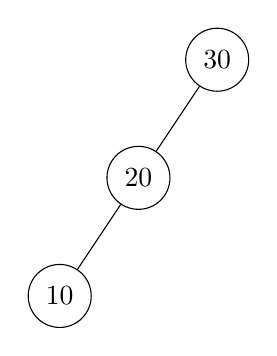
\begin{tikzpicture}[
                level distance=1.5cm,
                sibling distance=2cm,
                every node/.style={circle, draw, minimum size=0.8cm}
                ]
                % Unbalanced tree
                \node {30}
                child {node {20}
                    child {node {10}}
                    child[missing]
                }
                child[missing];
            \end{tikzpicture}
            \qquad
            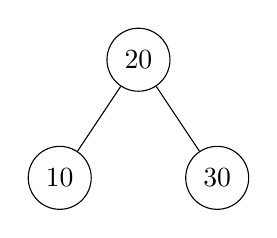
\begin{tikzpicture}[
                level distance=1.5cm,
                sibling distance=2cm,
                every node/.style={circle, draw, minimum size=0.8cm}
                ]
                % After right rotation
                \node {20}
                child {node {10}}
                child {node {30}};
            \end{tikzpicture}
        \end{latin}
        \caption{چرخش راست: گره ۲۰ به ریشه تبدیل می‌شود}
        \label{fig:right-rotation}
    \end{figure}
    
    \subsection{پیاده‌سازی}
    
    \begin{latin}
        \begin{minted}{python}
            from dataclasses import dataclass
            from typing import Optional
            
            
            @dataclass
            class AVLNode:
            key: int
            height: int = 1
            left: Optional['AVLNode'] = None
            right: Optional['AVLNode'] = None
            
            
            class AVLTree:
            """Self-balancing AVL tree implementation."""
            
            def height(self, node: Optional[AVLNode]) -> int:
            return node.height if node else 0
            
            def balance_factor(self, node: Optional[AVLNode]) -> int:
            return self.height(node.left) - self.height(node.right)
            
            def rotate_right(self, y: AVLNode) -> AVLNode:
            x = y.left
            T2 = x.right
            x.right = y
            y.left = T2
            y.height = 1 + max(self.height(y.left), self.height(y.right))
            x.height = 1 + max(self.height(x.left), self.height(x.right))
            return x
            
            def rotate_left(self, x: AVLNode) -> AVLNode:
            y = x.right
            T2 = y.left
            y.left = x
            x.right = T2
            x.height = 1 + max(self.height(x.left), self.height(x.right))
            y.height = 1 + max(self.height(y.left), self.height(y.right))
            return y
            
            def insert(self, node: Optional[AVLNode], key: int) -> AVLNode:
            """Insert a key and rebalance the tree."""
            if not node:
            return AVLNode(key)
            
            if key < node.key:
            node.left = self.insert(node.left, key)
            elif key > node.key:
            node.right = self.insert(node.right, key)
            else:
            return node  # Duplicate keys not allowed
            
            node.height = 1 + max(self.height(node.left),
            self.height(node.right))
            
            balance = self.balance_factor(node)
            
            # Left-Left case
            if balance > 1 and key < node.left.key:
            return self.rotate_right(node)
            # Right-Right case
            if balance < -1 and key > node.right.key:
            return self.rotate_left(node)
            # Left-Right case
            if balance > 1 and key > node.left.key:
            node.left = self.rotate_left(node.left)
            return self.rotate_right(node)
            # Right-Left case
            if balance < -1 and key < node.right.key:
            node.right = self.rotate_right(node.right)
            return self.rotate_left(node)
            
            return node
        \end{minted}
    \end{latin}
    \codecaption{درخت AVL با چرخش‌های خودکار}
    \label{code:avl}
    
    \section{درخت سرخ-سیاه}
    
    \subsection{تعریف}
    
    \begin{definition}[درخت سرخ-سیاه]
        یک درخت جستجوی دودویی که هر گره آن
        دارای یک \textbf{رنگ}\index{درخت سرخ-سیاه}
        (قرمز یا سیاه) است و پنج شرط زیر برقرار است:
        \begin{enumerate}
            \item هر گره یا قرمز است یا سیاه
            \item ریشه همواره سیاه است
            \item برگ‌های NIL سیاه هستند
            \item فرزندان یک گره قرمز، سیاه هستند
            \item تعداد گره‌های سیاه در مسیر از هر گره
            به برگ‌های NIL یکسان است
        \end{enumerate}
        \label{def:red-black}
    \end{definition}
    
    \begin{theorem}[ارتفاع درخت سرخ-سیاه]
        ارتفاع درخت سرخ-سیاه با $n$ کلید
        حداکثر $2\log_{2}(n+1)$ است.
        \label{thm:rb-height}
    \end{theorem}
    
    \subsection{عملیات درج}
    
    درج در درخت سرخ-سیاه شامل سه گام است:
    \begin{enumerate}
        \item درج مانند BST معمولی (گره جدید قرمز)
        \item رنگ‌آمیزی مجدد برای حفظ شرایط
        \item چرخش در صورت نیاز
    \end{enumerate}
    
    حالت‌های نقض شرط ۴ (پدر و عمو قرمز،
    عمو سیاه با ساختار مثلثی یا خطی).
    
    \begin{remark}
        درخت سرخ-سیاه در کتابخانه‌های استاندارد
        مانند \texttt{std::map} در C++ و
        \texttt{TreeMap} در جاوا استفاده می‌شود.
        دلیل انتخاب آن نسبت به AVL،
        تعداد کمتر چرخش‌ها در عملیات درج است.
        \label{rem:rb-vs-avl}
    \end{remark}
    
    \section{درخت B و B+}
    
    \subsection{انگیزه}
    
    برای داده‌های حجیم که در حافظه جا نمی‌شوند
    و روی دیسک\index{پایگاه داده} ذخیره می‌شوند،
    تعداد دسترسی‌های دیسک عامل تعیین‌کننده است.
    درخت B\index{درخت B} با افزایش ضریب انشعاب،
    ارتفاع را کاهش می‌دهد.
    
    \begin{definition}[درخت B از مرتبه $t$]
        \begin{itemize}
            \item هر گره (جز ریشه) حداقل $t-1$ کلید دارد
            \item هر گره حداکثر $2t-1$ کلید دارد
            \item هر گره با $k$ کلید، $k+1$ فرزند دارد
            \item تمام برگ‌ها در یک سطح هستند
        \end{itemize}
        \label{def:b-tree}
    \end{definition}
    
    ارتفاع درخت B با $n$ کلید:
    $h \leq \log_{t} \frac{n+1}{2}$
    
    \begin{figure}[h]
        \centering
        \begin{latin}
            \begin{tikzpicture}[
                level distance=1.8cm,
                sibling distance=3cm,
                bnode/.style={rectangle, draw=matindarkblue, fill=matinlightblue!30,
                    rounded corners, minimum width=4cm, minimum height=0.8cm}
                ]
                \node[bnode] {20 | 40 | 60}
                child {node[bnode] {5 | 10}}
                child {node[bnode] {25 | 30 | 35}}
                child {node[bnode] {45 | 50}}
                child {node[bnode] {70 | 80 | 90}};
            \end{tikzpicture}
        \end{latin}
        \caption{درخت B از مرتبه $t=3$ (درخت ۲-۳-۴)}
        \label{fig:b-tree}
    \end{figure}
    
    \subsection{درخت B+}
    
    \begin{definition}[درخت B+]
        مشابه درخت B، با دو تفاوت:
        \begin{enumerate}
            \item تمام کلیدها در برگ‌ها ذخیره می‌شوند
            (گره‌های داخلی فقط راهنما هستند)
            \item برگ‌ها به صورت لیست پیوندی
            به هم متصل شده‌اند
        \end{enumerate}
        \label{def:b-plus-tree}
    \end{definition}
    
    مزیت اصلی: پیمایش ترتیبی بسیار سریع
    و مناسب برای \textbf{پرس‌وجوهای بازه‌ای}
    در پایگاه داده.
    
    \section{درخت‌های تصادفی}
    
    \subsection{Treap}
    
    \begin{definition}[Treap]
        ترکیب \textbf{Tree} + \textbf{Heap}.
        هر گره یک کلید (طبق BST) و یک
        \textbf{اولویت تصادفی} (طبق Max-Heap) دارد.
        اولویت‌های تصادفی تضمین می‌کنند
        ارتفاع مورد انتظار $O(\log n)$ باشد.
        \label{def:treap}
    \end{definition}
    
    مزیت: پیاده‌سازی بسیار ساده‌تر از AVL
    و سرخ-سیاه. درج و حذف تنها با چرخش.
    
    \subsection{درخت جستجوی تصادفی}
    
    اگر عناصر را به ترتیب \textbf{تصادفی}
    در یک BST ساده درج کنیم،
    ارتفاع مورد انتظار $O(\log n)$ خواهد بود.
    این نتیجه از تحلیل Quick Sort می‌آید.
    
    \section{تحلیل پیچیدگی}
    
    \begin{table}[h]
        \centering
        \caption{پیچیدگی عملیات در درخت‌های متوازن}
        \label{tab:tree-complexity}
        \begin{tabular}{|c|c|c|c|c|}
            \hline
            \textbf{عملیات} & \textbf{AVL} & \textbf{سرخ-سیاه} & \textbf{B-Tree} & \textbf{Treap} \\
            \hline
            جستجو & $O(\log n)$ & $O(\log n)$ & $O(\log_{t} n)$ & $O(\log n)$* \\
            درج & $O(\log n)$ & $O(\log n)$ & $O(\log_{t} n)$ & $O(\log n)$* \\
            حذف & $O(\log n)$ & $O(\log n)$ & $O(\log_{t} n)$ & $O(\log n)$* \\
            چرخش در درج & $\leq 2$ & $\leq 2$ & تقسیم & $\leq 2$* \\
            چرخش در حذف & $O(\log n)$ & $\leq 3$ & ادغام & $O(\log n)$* \\
            \hline
        \end{tabular}
    \end{table}
    * مورد انتظار، نه بدترین حالت
    
    \section{تمرین‌ها}
    
    \begin{exercise}
        یک درخت AVL اولیه خالی را در نظر بگیرید.
        اعداد $10, 20, 30, 40, 50, 25$ را
        به ترتیب درج کنید و پس از هر درج،
        ساختار درخت را رسم کنید.
        \label{exc:avl-insert-sequence}
    \end{exercise}
    
    \begin{exercise}
        ثابت کنید ارتفاع درخت سرخ-سیاه
        با $n$ کلید داخلی حداکثر
        $2\log_{2}(n+1)$ است.
        \label{exc:rb-height-proof}
    \end{exercise}
    
    \begin{exercise}
        نشان دهید چرا درخت B برای ذخیره‌سازی
        روی دیسک مناسب‌تر از درخت دودویی است.
        زمان دسترسی به دیسک را $10$ میلی‌ثانیه
        و زمان پردازش در حافظه را $0.1$ میکروثانیه
        فرض کنید.
        \label{exc:b-tree-disk}
    \end{exercise}
    
    \begin{exercise}
        یک \lr{Treap} پیاده‌سازی کنید
        و ارتفاع آن را برای $n = 1000$ درج تصادفی
        به طور تجربی اندازه بگیرید.
        آزمایش را ۱۰۰ بار تکرار و میانگین را گزارش کنید.
        \label{exc:treap-experiment}
    \end{exercise}
    
    \begin{exercise}
        الگوریتم \textbf{ادغام} دو درخت AVL
        با پیچیدگی $O(\log n)$ را طراحی کنید.
        \label{exc:avl-merge}
    \end{exercise}
    
    %========================================
    % MatinBook - Advanced Algorithms & Mathematics
    % Chapter 6: Advanced Heap Data Structures
    %========================================
    
    \chapter{هیپ‌های پیشرفته}
    \label{chap:advanced-heaps}
    
    \section{مقدمه}
    
    هیپ\index{هیپ} یکی از پرکاربردترین ساختمان داده‌ها
    در علوم کامپیوتر است. هیپ دودویی ساده
    عملیات درج و حذف کمینه را در $O(\log n)$
    انجام می‌دهد، اما برای برخی کاربردها
    (مانند الگوریتم دایکسترا با کاهش کلید،
    یا ادغام دو صف اولویت) ناکافی است.
    در این فصل، هیپ‌های پیشرفته‌ای را بررسی می‌کنیم
    که این عملیات را کاراتر انجام می‌دهند.
    
    \begin{definition}[هیپ]
        یک \textbf{هیپ} درختی است که در آن
        هر گره دارای کلیدی کوچک‌تر (یا بزرگ‌تر)
        از فرزندانش است (\textbf{خاصیت هیپ}).
        \label{def:heap}
    \end{definition}
    
    \begin{table}[h]
        \centering
        \caption{مقایسه انواع هیپ‌ها}
        \label{tab:heap-comparison}
        \begin{tabular}{|c|C{2.5cm}|C{2.5cm}|C{2.5cm}|C{2.5cm}|}
            \hline
            \textbf{عملیات} & \textbf{دودویی} & \textbf{دوجمله‌ای} & \textbf{فیبوناچی} & \textbf{چپ‌گرا} \\
            \hline
            درج & $O(\log n)$ & $O(\log n)$ & $O(1)$ & $O(\log n)$ \\
            حذف کمینه & $O(\log n)$ & $O(\log n)$ & $O(\log n)$* & $O(\log n)$ \\
            کاهش کلید & $O(\log n)$ & $O(\log n)$ & $O(1)$* & $O(\log n)$ \\
            ادغام & $O(n)$ & $O(\log n)$ & $O(1)$ & $O(\log n)$ \\
            \hline
        \end{tabular}
    \end{table}
    * تحلیل سرشکن
    
    \section{هیپ دوجمله‌ای}
    
    \subsection{درخت دوجمله‌ای}
    
    \begin{definition}[درخت دوجمله‌ای]
        درخت دوجمله‌ای\index{درخت دوجمله‌ای}
        $B_{k}$ به صورت بازگشتی تعریف می‌شود:
        \begin{itemize}
            \item $B_{0}$: یک گره منفرد
            \item $B_{k}$: از اتصال دو درخت $B_{k-1}$
            ساخته می‌شود، یکی به عنوان فرزند ریشه دیگری
        \end{itemize}
        \label{def:binomial-tree}
    \end{definition}
    
    ویژگی‌های $B_{k}$:
    \begin{itemize}
        \item تعداد گره‌ها: $2^{k}$
        \item ارتفاع: $k$
        \item تعداد فرزندان ریشه: $k$
        \item تعداد گره‌ها در عمق $d$: $\binom{k}{d}$
    \end{itemize}
    
    \subsection{هیپ دوجمله‌ای}
    
    \begin{definition}[هیپ دوجمله‌ای]
        مجموعه‌ای از درخت‌های دوجمله‌ای
        که هر کدام خاصیت هیپ دارند و
        حداکثر یک درخت از هر مرتبه $k$ وجود دارد.
        \label{def:binomial-heap}
    \end{definition}
    
    نمایش دودویی عدد $n$ مشخص می‌کند
    کدام درخت‌ها در هیپ حضور دارند.
    
    \begin{latin}
        \begin{algorithm}
            \begin{algorithmic}[1]
                \Function{Merge}{$H_{1}$, $H_{2}$}
                \State $H \gets$ empty heap
                \State $carry \gets$ None
                \For{$k \gets 0$ \textbf{to} $\max(\text{degree}) + 1$}
                \State Combine trees of order $k$ from
                $H_{1}$, $H_{2}$, and $carry$
                \State Store one tree in $H$,
                carry the other to next order
                \EndFor
                \State \Return $H$
                \EndFunction
            \end{algorithmic}
        \end{algorithm}
        \algcaption[alg:binomial-merge]{ادغام دو هیپ دوجمله‌ای}
    \end{latin}
    
    \subsection{تحلیل پیچیدگی}
    
    \begin{theorem}[زمان عملیات هیپ دوجمله‌ای]
        در هیپ دوجمله‌ای با $n$ عنصر:
        \begin{itemize}
            \item درج: $O(\log n)$ سرشکن
            \item حذف کمینه: $O(\log n)$
            \item کاهش کلید: $O(\log n)$
            \item ادغام: $O(\log n)$
        \end{itemize}
        \label{thm:binomial-complexity}
    \end{theorem}
    
    \section{هیپ فیبوناچی}
    
    \subsection{ساختار}
    
    هیپ فیبوناچی\index{هیپ فیبوناچی}
    (\lr{Fibonacci Heap}) توسط فردمن و تارجان
    در سال ۱۹۸۴ معرفی شد و پیچیدگی سرشکن
    بهتری برای عملیات کاهش کلید ارائه می‌دهد.
    
    \begin{definition}[هیپ فیبوناچی]
        مجموعه‌ای از درخت‌های ریشه‌دار
        با خاصیت هیپ کمینه است که
        \textbf{تنها} در زمان حذف کمینه
        بازسازی می‌شوند (\lr{lazy consolidation}).
        \label{def:fibonacci-heap}
    \end{definition}
    
    ویژگی‌های کلیدی:
    \begin{itemize}
        \item هر گره دارای نشانه \textbf{علامت‌گذاری}
        (\lr{mark}) برای ردیابی حذف فرزندان
        \item ریشه‌ها در یک \textbf{لیست دایره‌ای}
        نگهداری می‌شوند
        \item اشاره‌گر به کمینه همواره برقرار است
    \end{itemize}
    
    \subsection{عملیات و تحلیل سرشکن}
    
    \begin{theorem}[تحلیل فیبوناچی]
        با تابع پتانسیل
        $\Phi = t + 2m$
        که $t$ تعداد درخت‌ها و $m$ تعداد
        گره‌های علامت‌گذاری‌شده است:
        \begin{itemize}
            \item درج: $O(1)$ سرشکن
            \item کاهش کلید: $O(1)$ سرشکن
            \item حذف کمینه: $O(\log n)$ سرشکن
        \end{itemize}
        \label{thm:fibonacci-amortized}
    \end{theorem}
    
    \begin{proof}[ایده تحلیل کاهش کلید]
        کاهش کلید ممکن است باعث \textbf{برش}
        (\lr{cut}) گره از پدرش شود.
        اگر پدر قبلاً علامت‌گذاری شده باشد،
        آن نیز برش می‌خورد و این کار
        به صورت آبشاری ادامه می‌یابد.
        تحلیل سرشکن نشان می‌دهد هزینه هر برش
        توسط کاهش پتانسیل جبران می‌شود.
    \end{proof}
    
    \begin{remark}
        هیپ فیبوناچی از نظر تئوری عالی است،
        اما پیاده‌سازی پیچیده و ثابت‌های بزرگ
        باعث شده در عمل کمتر از هیپ دودویی
        یا دوجمله‌ای استفاده شود.
        کاربرد اصلی آن در الگوریتم‌های گراف
        با تعداد زیادی کاهش کلید است.
        \label{rem:fibonacci-practical}
    \end{remark}
    
    \subsection{کاربرد در الگوریتم دایکسترا}
    
    با هیپ فیبوناچی، الگوریتم دایکسترا
    از $O((V+E)\log V)$ به
    $O(V \log V + E)$ بهبود می‌یابد
    که برای گراف‌های چگال
    ($E = \Omega(V^{2})$) تفاوت چشمگیری دارد.
    
    \section{هیپ چپ‌گرا}
    
    \subsection{تعریف}
    
    \begin{definition}[هیپ چپ‌گرا]
        یک درخت دودویی با خاصیت هیپ که در آن
        \textbf{طول مسیر تهی}\index{طول مسیر تهی}
        (\lr{Null Path Length}) فرزند چپ
        همواره بزرگتر یا مساوی فرزند راست است.
        \label{def:leftist-heap}
    \end{definition}
    
    \begin{definition}[NPL]
        $NPL(x)$ کوتاه‌ترین فاصله از $x$
        تا یک گره با کمتر از دو فرزند است.
        $NPL(\text{null}) = -1$
        \label{def:npl}
    \end{definition}
    
    \subsection{ادغام}
    
    عملیات اصلی در هیپ چپ‌گرا،
    \textbf{ادغام}\index{ادغام} دو هیپ است.
    سایر عملیات بر اساس ادغام تعریف می‌شوند.
    
    \begin{latin}
        \begin{algorithm}
            \begin{algorithmic}[1]
                \Function{Merge}{$h_{1}$, $h_{2}$}
                \If{$h_{1} = \text{null}$}
                \State \Return $h_{2}$
                \EndIf
                \If{$h_{2} = \text{null}$}
                \State \Return $h_{1}$
                \EndIf
                \If{$h_{1}.\text{key} > h_{2}.\text{key}$}
                \State Swap $h_{1}$ and $h_{2}$
                \EndIf
                \State $h_{1}.\text{right} \gets
                \Call{Merge}{h_{1}.\text{right}, h_{2}}$
                \If{$NPL(h_{1}.\text{left}) < NPL(h_{1}.\text{right})$}
                \State Swap children of $h_{1}$
                \EndIf
                \State $NPL(h_{1}) \gets NPL(h_{1}.\text{right}) + 1$
                \State \Return $h_{1}$
                \EndFunction
            \end{algorithmic}
        \end{algorithm}
        \algcaption[alg:leftist-merge]{ادغام دو هیپ چپ‌گرا}
    \end{latin}
    
    \begin{theorem}[تحلیل هیپ چپ‌گرا]
        تمام عملیات در هیپ چپ‌گرا
        در بدترین حالت $O(\log n)$ هستند.
        \label{thm:leftist-complexity}
    \end{theorem}
    
    \subsection{پیاده‌سازی}
    
    \begin{latin}
        \begin{minted}{python}
            from dataclasses import dataclass
            from typing import Optional
            
            
            @dataclass
            class LeftistNode:
            key: int
            npl: int = 0
            left: Optional['LeftistNode'] = None
            right: Optional['LeftistNode'] = None
            
            
            def merge(h1: Optional[LeftistNode],
            h2: Optional[LeftistNode]) -> Optional[LeftistNode]:
            """Merge two leftist heaps."""
            if not h1:
            return h2
            if not h2:
            return h1
            if h1.key > h2.key:
            h1, h2 = h2, h1
            
            h1.right = merge(h1.right, h2)
            
            left_npl = h1.left.npl if h1.left else -1
            right_npl = h1.right.npl if h1.right else -1
            
            if left_npl < right_npl:
            h1.left, h1.right = h1.right, h1.left
            
            h1.npl = (h1.right.npl if h1.right else -1) + 1
            return h1
            
            
            def insert(h: Optional[LeftistNode], key: int):
            """Insert a key into the heap."""
            return merge(h, LeftistNode(key))
            
            
            def extract_min(h: Optional[LeftistNode]):
            """Remove and return the minimum key."""
            if not h:
            return None, None
            return h.key, merge(h.left, h.right)
        \end{minted}
    \end{latin}
    \codecaption{پیاده‌سازی هیپ چپ‌گرا}
    \label{code:leftist-heap}
    
    \section{هیپ‌های نرم}
    
    \subsection{هیپ دو-سه}
    
    هیپ دو-سه\index{هیپ دو-سه}
    (\lr{2-3 Heap}) یک ساختمان داده
    متوازن و ساده برای صف اولویت است
    که توسط Tadao Takaoka معرفی شد.
    
    \begin{definition}[هیپ دو-سه]
        درختی که هر گره دارای ۲ یا ۳ فرزند است
        و برگ‌ها در یک سطح قرار دارند.
        کلید هر گره از کلیدهای فرزندانش
        کوچک‌تر است.
        \label{def:2-3-heap}
    \end{definition}
    
    \subsection{هیپ Pairing}
    
    هیپ Pairing\index{هیپ Pairing}
    یک هیپ ساده و کارا در عمل است که
    تحلیل نظری پیچیده‌ای دارد.
    
    \begin{definition}[هیپ Pairing]
        یک درخت با خاصیت هیپ که
        عملیات ادغام دو هیپ به سادگی
        با مقایسه ریشه‌ها انجام می‌شود.
        \label{def:pairing-heap}
    \end{definition}
    
    \begin{remark}
        هیپ Pairing در عمل از هیپ فیبوناچی
        سریع‌تر است، با این که تحلیل سرشکن
        آن $O(\log n)$ برای حذف کمینه
        (و نه $O(1)$) است.
        \label{rem:pairing-vs-fibonacci}
    \end{remark}
    
    \section{کاربردهای پیشرفته}
    
    \subsection{الگوریتم پریم با هیپ فیبوناچی}
    
    الگوریتم پریم\index{پریم} برای درخت
    پوشای کمینه با هیپ فیبوناچی
    در $O(E + V \log V)$ اجرا می‌شود.
    
    \subsection{کوتاه‌ترین مسیر با کاهش کلید}
    
    در الگوریتم دایکسترا،
    عملیات کاهش کلید تا $E$ بار
    فراخوانی می‌شود. با هیپ فیبوناچی،
    این عملیات عملاً رایگان است.
    
    \subsection{مرتب‌سازی خارجی}
    
    برای مرتب‌سازی داده‌های حجیم روی دیسک،
    از \textbf{مرتب‌سازی چندمسیره} استفاده می‌شود
    که هیپ کمینه با قابلیت ادغام سریع
    (مانند هیپ دوجمله‌ای) در آن کاربرد دارد.
    
    \section{تمرین‌ها}
    
    \begin{exercise}
        یک هیپ دوجمله‌ای پیاده‌سازی کنید
        و نشان دهید که درج $n$ عنصر تصادفی
        هزینه سرشکن $O(1)$ دارد
        (با استفاده از تحلیل تجمیعی
        و مقایسه با جمع دودویی).
        \label{exc:binomial-insert-amortized}
    \end{exercise}
    
    \begin{exercise}
        ثابت کنید حداکثر درجه یک گره
        در هیپ فیبوناچی با $n$ عنصر
        $O(\log n)$ است.
        \label{exc:fibonacci-degree}
    \end{exercise}
    
    \begin{exercise}
        الگوریتم دایکسترا را یک بار با هیپ دودویی
        و بار دیگر با هیپ فیبوناچی پیاده‌سازی کنید
        و زمان اجرا را روی گراف‌های چگال
        ($E \approx V^{2}/2$) مقایسه کنید.
        \label{exc:dijkstra-heap-comparison}
    \end{exercise}
    
    \begin{exercise}
        نشان دهید عملیات \textbf{افزایش کلید}
        در هیپ فیبوناچی را می‌توان با
        حذف و درج مجدد در $O(\log n)$
        انجام داد. آیا روش کاراتری وجود دارد؟
        \label{exc:increase-key}
    \end{exercise}
    
    \begin{exercise}
        الگوریتم \textbf{مرتب‌سازی هیپی}
        (\lr{Heapsort}) را با استفاده از
        هیپ چپ‌گرا پیاده‌سازی کنید.
        \label{exc:heapsort-leftist}
    \end{exercise}
    
    
    %========================================
    % MatinBook - Advanced Algorithms & Mathematics
    % Chapter 7: Disjoint Set Union and Amortized Analysis
    %========================================
    
    \chapter{ساختمان داده برای مجموعه‌های مجزا}
    \label{chap:union-find}
    
    \section{مقدمه}
    
    ساختمان داده \textbf{مجموعه‌های مجزا}\index{مجموعه‌های مجزا}
    (\lr{Disjoint Set Union} یا \lr{Union-Find})
    یکی از ساده‌ترین و در عین حال قدرتمندترین
    ساختمان داده‌ها در علوم کامپیوتر است.
    این ساختمان داده، افرازی از یک مجموعه
    را به صورت پویا مدیریت می‌کند.
    
    \begin{definition}[مجموعه‌های مجزا]
        یک افراز از مجموعه $U = \{1, 2, \ldots, n\}$
        به زیرمجموعه‌های ناتهی و جدا از هم
        که اجتماع آن‌ها $U$ می‌شود.
        \label{def:disjoint-sets}
    \end{definition}
    
    \subsection{عملیات اصلی}
    
    \begin{definition}[عملیات Union-Find]
        سه عملیات اصلی:
        \begin{enumerate}
            \item \textbf{MakeSet(x):}
            مجموعه‌ای تک‌عضوی شامل $x$ ایجاد کن
            \item \textbf{Find(x):}
            نماینده (ریشه) مجموعه حاوی $x$ را برگردان
            \item \textbf{Union(x, y):}
            دو مجموعه حاوی $x$ و $y$ را ادغام کن
        \end{enumerate}
        \label{def:union-find-operations}
    \end{definition}
    
    \subsection{کاربردها}
    
    \begin{itemize}
        \item \textbf{الگوریتم کروسکال:}
        برای تشخیص دور در ساخت درخت پوشای کمینه
        \item \textbf{اتصال در گراف:}
        بررسی پویای همبندی گراف
        \item \textbf{پردازش تصویر:}
        برچسب‌گذاری مؤلفه‌های همبند
        \item \textbf{بازی‌سازی:}
        تشخیص گروه‌های همبند در صفحه بازی
    \end{itemize}
    
    \section{پیاده‌سازی پایه}
    
    \subsection{نمایش با جنگل}
    
    هر مجموعه را با یک \textbf{درخت ریشه‌دار}
    نمایش می‌دهیم. ریشه درخت، \textbf{نماینده}
    مجموعه است. هر گره به پدرش اشاره می‌کند.
    
    \begin{latin}
        \begin{minted}{python}
            class DSU:
            """Basic Disjoint Set Union implementation."""
            
            def __init__(self, n: int):
            self.parent = list(range(n))
            
            def find(self, x: int) -> int:
            """Find representative of set containing x."""
            while self.parent[x] != x:
            x = self.parent[x]
            return x
            
            def union(self, x: int, y: int) -> None:
            """Merge sets containing x and y."""
            root_x = self.find(x)
            root_y = self.find(y)
            if root_x != root_y:
            self.parent[root_x] = root_y
        \end{minted}
    \end{latin}
    \codecaption{پیاده‌سازی پایه Union-Find}
    \label{code:dsu-basic}
    
    \begin{remark}
        در این پیاده‌سازی ساده،
        عملیات \texttt{Find} در بدترین حالت $O(n)$
        و \texttt{Union} نیز $O(n)$ است،
        زیرا درخت می‌تواند به یک زنجیره تبدیل شود.
        \label{rem:dsu-basic-worst}
    \end{remark}
    
    \section{بهبود با اجتماع بر اساس رتبه}
    
    \subsection{ایده}
    
    برای جلوگیری از ایجاد درخت‌های طویل،
    هنگام ادغام، ریشه درخت \textbf{کوتاه‌تر} را
    فرزند ریشه درخت \textbf{بلندتر} قرار می‌دهیم.
    
    \begin{definition}[رتبه]
        \textbf{رتبه}\index{رتبه} (\lr{rank}) یک گره
        تخمینی از ارتفاع زیردرخت آن است.
        \label{def:rank}
    \end{definition}
    
    \begin{latin}
        \begin{algorithm}
            \begin{algorithmic}[1]
                \Function{Union}{$x$, $y$}
                \State $rootX \gets \Call{Find}{x}$
                \State $rootY \gets \Call{Find}{y}$
                \If{$rootX = rootY$}
                \State \Return
                \EndIf
                \If{$rank[rootX] < rank[rootY]$}
                \State $parent[rootX] \gets rootY$
                \ElsIf{$rank[rootX] > rank[rootY]$}
                \State $parent[rootY] \gets rootX$
                \Else
                \State $parent[rootY] \gets rootX$
                \State $rank[rootX] \gets rank[rootX] + 1$
                \EndIf
                \EndFunction
            \end{algorithmic}
        \end{algorithm}
        \algcaption[alg:union-rank]{اجتماع با رتبه}
    \end{latin}
    
    \subsection{تحلیل}
    
    \begin{theorem}[ارتفاع با اجتماع بر اساس رتبه]
        با استفاده از اجتماع بر اساس رتبه،
        ارتفاع هر درخت حداکثر $\lfloor \log_{2} n \rfloor$ است.
        \label{thm:union-rank-height}
    \end{theorem}
    
    \begin{proof}
        با استقرا روی تعداد عناصر.
        برای $n = 1$، ارتفاع ۰ است.
        هنگام ادغام دو درخت با رتبه‌های $r_{1}$ و $r_{2}$،
        اگر $r_{1} < r_{2}$، ارتفاع تغییر نمی‌کند.
        اگر $r_{1} = r_{2} = r$، ارتفاع $r+1$ می‌شود
        و تعداد عناصر حداقل $2^{r+1}$ است.
    \end{proof}
    
    \section{فشرده‌سازی مسیر}
    
    \subsection{ایده}
    
    در حین \texttt{Find(x)}، تمام گره‌های
    مسیر از $x$ تا ریشه را \textbf{مستقیماً}
    به ریشه وصل می‌کنیم.
    
    \begin{definition}[فشرده‌سازی مسیر]
        \textbf{فشرده‌سازی مسیر}\index{فشرده‌سازی مسیر}
        (\lr{Path Compression}) یک تکنیک
        برای کاهش ارتفاع درخت است که در آن
        هر گره بازدیدشده در عملیات Find،
        فرزند مستقیم ریشه می‌شود.
        \label{def:path-compression}
    \end{definition}
    
    \begin{latin}
        \begin{minted}{python}
            def find(self, x: int) -> int:
            """Find with path compression."""
            if self.parent[x] != x:
            self.parent[x] = self.find(self.parent[x])
            return self.parent[x]
        \end{minted}
    \end{latin}
    \codecaption{Find با فشرده‌سازی مسیر}
    \label{code:find-path-compression}
    
    \subsection{تحلیل با تابع آکرمن}
    
    \begin{definition}[تابع آکرمن معکوس]
        تابع $\alpha(n)$ معکوس تابع آکرمن\index{آکرمن}
        است که بسیار کند رشد می‌کند:
        $\alpha(n) \leq 4$ برای تمام
        $n \leq 2^{2^{2^{2^{16}}}}$
        (تعداد اتم‌های جهان).
        \label{def:ackermann}
    \end{definition}
    
    \begin{theorem}[تحلیل تارجان]
        با استفاده از \textbf{اجتماع بر اساس رتبه}
        و \textbf{فشرده‌سازی مسیر}،
        هزینه سرشکن هر عملیات
        $O(\alpha(n))$ است
        که در عمل ثابت محسوب می‌شود.
        \label{thm:tarjan-union-find}
    \end{theorem}
    
    \begin{proof}[ایده اثبات]
        گره‌ها را بر اساس رتبه به بلوک‌هایی
        تقسیم می‌کنیم. تابع آکرمن معکوس
        تعداد دفعاتی که رتبه یک گره
        می‌تواند بلوک خود را تغییر دهد
        محدود می‌کند. تحلیل دقیق
        خارج از حوصله این کتاب است
        \cite{cormen2009}.
    \end{proof}
    
    \subsection{پیاده‌سازی کامل}
    
    \begin{latin}
        \begin{minted}{python}
            class DSU:
            """Optimized DSU with union by rank and path compression."""
            
            def __init__(self, n: int):
            self.parent = list(range(n))
            self.rank = [0] * n
            self.components = n  # Number of disjoint sets
            
            def find(self, x: int) -> int:
            """Find representative with path compression."""
            if self.parent[x] != x:
            self.parent[x] = self.find(self.parent[x])
            return self.parent[x]
            
            def union(self, x: int, y: int) -> bool:
            """
            Merge sets containing x and y.
            Returns True if merge happened, False if already same set.
            """
            root_x = self.find(x)
            root_y = self.find(y)
            
            if root_x == root_y:
            return False
            
            if self.rank[root_x] < self.rank[root_y]:
            root_x, root_y = root_y, root_x
            
            self.parent[root_y] = root_x
            
            if self.rank[root_x] == self.rank[root_y]:
            self.rank[root_x] += 1
            
            self.components -= 1
            return True
            
            def is_same(self, x: int, y: int) -> bool:
            """Check if x and y are in the same set."""
            return self.find(x) == self.find(y)
        \end{minted}
    \end{latin}
    \codecaption{پیاده‌سازی کامل DSU با بهینه‌سازی}
    \label{code:dsu-optimized}
    
    \section{گونه‌های توسعه‌یافته}
    
    \subsection{DSU با وزن}
    
    در برخی مسائل، علاوه بر تشخیص مجموعه،
    به \textbf{اندازه} یا \textbf{مجموع} عناصر
    هر مجموعه نیز نیاز داریم.
    
    \begin{latin}
        \begin{minted}{python}
            class WeightedDSU:
            """DSU that tracks size of each component."""
            
            def __init__(self, n: int):
            self.parent = list(range(n))
            self.size = [1] * n
            
            def find(self, x: int) -> int:
            if self.parent[x] != x:
            self.parent[x] = self.find(self.parent[x])
            return self.parent[x]
            
            def union(self, x: int, y: int) -> bool:
            root_x = self.find(x)
            root_y = self.find(y)
            if root_x == root_y:
            return False
            if self.size[root_x] < self.size[root_y]:
            root_x, root_y = root_y, root_x
            self.parent[root_y] = root_x
            self.size[root_x] += self.size[root_y]
            return True
            
            def get_size(self, x: int) -> int:
            """Return size of component containing x."""
            return self.size[self.find(x)]
        \end{minted}
    \end{latin}
    \codecaption{DSU با ردیابی اندازه مجموعه}
    \label{code:dsu-weighted}
    
    \subsection{DSU با فاصله تا ریشه}
    
    در برخی کاربردها، نیاز داریم
    فاصله (یا مجموع وزن‌های) یک عنصر
    تا نماینده مجموعه را بدانیم.
    
    \subsection{Union-Find پایا}
    
    \begin{definition}[Union-Find پایا]
        نسخه‌ای که تمام تاریخچه ادغام‌ها
        را حفظ می‌کند و امکان پرس‌وجو
        درباره وضعیت در زمان‌های گذشته
        را فراهم می‌کند.
        \label{def:persistent-union-find}
    \end{definition}
    
    \section{کاربردها}
    
    \subsection{الگوریتم کروسکال}
    
    \begin{latin}
        \begin{minted}{python}
            def kruskal_mst(n: int, edges: list) -> list:
            """
            Compute Minimum Spanning Tree using Kruskal's algorithm.
            
            Args:
            n: Number of vertices.
            edges: List of (weight, u, v) tuples.
            
            Returns:
            List of edges in the MST.
            """
            dsu = DSU(n)
            edges.sort()  # Sort by weight
            mst = []
            
            for weight, u, v in edges:
            if dsu.union(u, v):
            mst.append((weight, u, v))
            if len(mst) == n - 1:
            break
            
            return mst
        \end{minted}
    \end{latin}
    \codecaption{الگوریتم کروسکال با DSU}
    \label{code:kruskal}
    
    \subsection{همبندی پویا در گراف}
    
    با اضافه شدن تدریجی یال‌ها به گراف،
    می‌توان تعداد مؤلفه‌های همبند را
    در هر لحظه با DSU ردیابی کرد.
    
    \subsection{LCA با الگوریتم تارجان}
    
    پیدا کردن \textbf{کمترین جد مشترک}
    (\lr{Lowest Common Ancestor}) در درخت
    با استفاده از DSU و پیمایش DFS
    در $O(n + q \cdot \alpha(n))$.
    
    \section{تمرین‌ها}
    
    \begin{exercise}
        ثابت کنید با اجتماع بر اساس رتبه
        (بدون فشرده‌سازی مسیر)،
        عملیات Find در $O(\log n)$
        و Union در $O(1)$ انجام می‌شود.
        \label{exc:union-rank-log}
    \end{exercise}
    
    \begin{exercise}
        یک \lr{Union-Find} پیاده‌سازی کنید
        که بتواند تعداد عناصر هر مجموعه را
        در $O(\alpha(n))$ برگرداند.
        \label{exc:dsu-size}
    \end{exercise}
    
    \begin{exercise}
        مسئله \textbf{بزرگ‌ترین مؤلفه همبند}
        در یک شبکه پویا را با DSU حل کنید.
        در ابتدا $n$ گره بدون یال داریم.
        یال‌ها یک به یک اضافه می‌شوند.
        پس از هر اضافه، اندازه بزرگ‌ترین
        مؤلفه را چاپ کنید.
        \label{exc:largest-component}
    \end{exercise}
    
    \begin{exercise}
        با استفاده از Union-Find،
        الگوریتمی برای تشخیص آنلاین
        \textbf{دور} در گراف نامرتبط
        طراحی کنید.
        \label{exc:cycle-detection}
    \end{exercise}
    
    \begin{exercise}
        ثابت کنید هزینه سرشکن $m$ عملیات
        روی DSU با اجتماع بر اساس رتبه
        و فشرده‌سازی مسیر،
        $O(m \cdot \alpha(n))$ است.
        (راهنمایی: از تحلیل بلوکی
        تابع آکرمن استفاده کنید.)
        \label{exc:tarjan-proof}
    \end{exercise}
    
    
    %========================================
    % MatinBook - Advanced Algorithms & Mathematics
    % Chapter 8: Suffix Trees and String Algorithms
    %========================================
    
    \chapter{درخت‌های پسوندی و الگوریتم‌های رشته‌ای}
    \label{chap:string-algorithms}
    
    \section{مقدمه}
    
    رشته‌ها\index{رشته} از بنیادی‌ترین انواع داده
    در علوم کامپیوتر هستند. از جستجوی الگو
    در DNA تا موتورهای جستجوی متن،
    الگوریتم‌های رشته‌ای\index{الگوریتم رشته‌ای}
    نقش حیاتی دارند. در این فصل،
    ساختمان داده‌های پیشرفته برای
    پردازش رشته‌ها را بررسی می‌کنیم.
    
    \section{درخت پیشوندی (Trie)}
    
    \subsection{تعریف و ساختار}
    
    \begin{definition}[Trie]
        \textbf{Trie}\index{Trie}
        (برگرفته از \lr{reTRIEval})
        یک درخت چندراهه است که در آن
        هر گره نمایش‌دهنده یک پیشوند
        از رشته‌های ذخیره‌شده است.
        یال‌ها با کاراکترها برچسب‌گذاری می‌شوند.
        \label{def:trie}
    \end{definition}
    
    \begin{figure}[h]
        \centering
        \begin{latin}
            \begin{tikzpicture}[
                level distance=1.5cm,
                sibling distance=2cm,
                trienode/.style={circle, draw=matinblue, fill=matinlightblue!30,
                    minimum size=0.8cm, font=\small},
                endnode/.style={circle, draw=matinred, fill=matinlightred!30,
                    minimum size=0.8cm, font=\small, double}
                ]
                \node[trienode] {}
                child {node[trienode] {a}
                    child {node[endnode] {n}
                        child {node[endnode] {t}}
                    }
                }
                child {node[trienode] {b}
                    child {node[trienode] {a}
                        child {node[endnode] {t}}
                        child {node[endnode] {g}}
                    }
                };
            \end{tikzpicture}
        \end{latin}
        \caption{Trie برای کلمات ant، bat، bag (گره‌های دوتایی = انتهای کلمه)}
        \label{fig:trie}
    \end{figure}
    
    \subsection{پیاده‌سازی}
    
    \begin{latin}
        \begin{minted}{python}
            from dataclasses import dataclass, field
            from typing import Dict, List, Optional
            
            
            @dataclass
            class TrieNode:
            children: Dict[str, 'TrieNode'] = field(default_factory=dict)
            is_end: bool = False
            value: Optional[str] = None
            
            
            class Trie:
            """Standard Trie implementation for string storage."""
            
            def __init__(self):
            self.root = TrieNode()
            
            def insert(self, word: str) -> None:
            """Insert a word into the Trie."""
            node = self.root
            for char in word:
            if char not in node.children:
            node.children[char] = TrieNode()
            node = node.children[char]
            node.is_end = True
            node.value = word
            
            def search(self, word: str) -> bool:
            """Check if word exists in the Trie."""
            node = self.root
            for char in word:
            if char not in node.children:
            return False
            node = node.children[char]
            return node.is_end
            
            def starts_with(self, prefix: str) -> List[str]:
            """Find all words with given prefix."""
            node = self.root
            for char in prefix:
            if char not in node.children:
            return []
            node = node.children[char]
            return self._collect_words(node)
            
            def _collect_words(self, node: TrieNode) -> List[str]:
            """Collect all complete words from subtree."""
            result = []
            if node.is_end:
            result.append(node.value)
            for child in node.children.values():
            result.extend(self._collect_words(child))
            return result
            
            
            # Usage
            trie = Trie()
            for word in ["cat", "car", "card", "care", "dog", "door"]:
            trie.insert(word)
            
            print(trie.search("car"))          # True
            print(trie.starts_with("ca"))      # ['cat', 'car', 'card', 'care']
        \end{minted}
    \end{latin}
    \codecaption{پیاده‌سازی Trie استاندارد}
    \label{code:trie}
    
    \subsection{Trie فشرده (Radix Tree)}
    
    \begin{definition}[Radix Tree]
        در \textbf{درخت ریشه}\index{Radix Tree}
        (\lr{Radix Tree} یا \lr{Patricia Trie})،
        زنجیره گره‌های تک‌فرزندی
        در یک گره فشرده می‌شوند.
        این کار حافظه مصرفی را
        به طور چشمگیری کاهش می‌دهد.
        \label{def:radix-tree}
    \end{definition}
    
    \subsection{کاربردهای Trie}
    
    \begin{itemize}
        \item \textbf{تکمیل خودکار:}
        پیشنهاد کلمات با پیشوند مشخص
        \item \textbf{غلط‌یاب:}
        تشخیص کلمات ناموجود در دیکشنری
        \item \textbf{مسیریابی IP:}
        جستجوی طولانی‌ترین پیشوند مشترک
        \item \textbf{XOR بیشینه:}
        یافتن دو عدد با بیشینه XOR
    \end{itemize}
    
    \section{درخت پسوندی (\lr{Suffix Tree})}
    
    \subsection{تعریف}
    
    \begin{definition}[درخت پسوندی]
        \textbf{درخت پسوندی}\index{درخت پسوندی}
        (\lr{Suffix Tree}) برای رشته $S$
        یک درخت فشرده از تمام
        $|S|$ پسوند $S$ است.
        \label{def:suffix-tree}
    \end{definition}
    
    برای رشته $S = \text{"banana\$"}$،
    پسوندها عبارتند از: \texttt{banana\$},
    \texttt{anana\$}, \texttt{nana\$},
    \texttt{ana\$}, \texttt{na\$}, \texttt{a\$}, \texttt{\$}.
    
    \begin{figure}[h]
        \centering
        \begin{latin}
            \begin{tikzpicture}[
                level distance=1.8cm,
                sibling distance=3cm,
                stnode/.style={rectangle, draw=matindarkblue, fill=matinlightblue!20,
                    rounded corners, minimum width=1.5cm, minimum height=0.7cm,
                    font=\ttfamily\small}
                ]
                \node[stnode] {root}
                child {node[stnode] {a}
                    child {node[stnode] {\$}
                        child {node[stnode, draw=matinred] {6}}
                    }
                    child {node[stnode] {na}
                        child {node[stnode] {\$}
                            child {node[stnode, draw=matinred] {4}}
                        }
                        child {node[stnode] {na\$}
                            child {node[stnode, draw=matinred] {2}}
                        }
                    }
                }
                child {node[stnode] {na}
                    child {node[stnode] {\$}
                        child {node[stnode, draw=matinred] {5}}
                    }
                    child {node[stnode] {na\$}
                        child {node[stnode, draw=matinred] {3}}
                    }
                };
            \end{tikzpicture}
        \end{latin}
        \caption{درخت پسوندی برای "banana\$" (نمایش ساده‌شده)}
        \label{fig:suffix-tree}
    \end{figure}
    
    \subsection{کاربردها}
    
    درخت پسوندی مسائل زیر را در $O(m)$
    حل می‌کند (که $m$ طول الگوست):
    
    \begin{itemize}
        \item \textbf{جستجوی الگو:}
        آیا الگو در متن وجود دارد؟
        \item \textbf{تعداد وقوع:}
        الگو چند بار ظاهر شده؟
        \item \textbf{طولانی‌ترین زیررشته مشترک:}
        بین دو رشته
        \item \textbf{طولانی‌ترین زیررشته تکراری:}
        در یک رشته
        \item \textbf{کوتاه‌ترین رشته منحصربه‌فرد:}
        رشته‌ای که فقط یک بار ظاهر شده
    \end{itemize}
    
    \subsection{الگوریتم اوکونن}
    
    الگوریتم اوکونن\index{اوکونن}
    (\lr{Ukkonen's Algorithm}) درخت پسوندی
    را در زمان $O(n)$ می‌سازد،
    که $n$ طول رشته است.
    
    \begin{remark}
        پیاده‌سازی درخت پسوندی پیچیده است
        و حافظه زیادی مصرف می‌کند
        ($\approx 20n$ بایت).
        \textbf{آرایه پسوندی}\index{آرایه پسوندی}
        (\lr{Suffix Array}) جایگزین
        فشرده‌تری است که همان کارایی
        مجانبی را با حافظه کمتر ارائه می‌دهد.
        \label{rem:suffix-tree-memory}
    \end{remark}
    
    \section{آرایه پسوندی و آرایه LCP}
    
    \subsection{آرایه پسوندی}
    
    \begin{definition}[آرایه پسوندی]
        \textbf{آرایه پسوندی}\index{آرایه پسوندی}
        (\lr{Suffix Array}) جایگشتی از
        اندیس‌های $0, 1, \ldots, n-1$ است
        که پسوندهای متناظر به ترتیب
        لغت‌نامه‌ای مرتب شده‌اند.
        \label{def:suffix-array}
    \end{definition}
    
    برای $S = \text{"banana"}$:
    \[
    SA = [5, 3, 1, 0, 4, 2]
    \]
    پسوندها: \texttt{a}, \texttt{ana}, \texttt{anana},
    \texttt{banana}, \texttt{na}, \texttt{nana}
    
    \subsection{آرایه LCP}
    
    \begin{definition}[آرایه LCP]
        \textbf{آرایه طولانی‌ترین پیشوند مشترک}
        (\lr{LCP Array}) طول طولانی‌ترین
        پیشوند مشترک بین دو پسوند متوالی
        در آرایه پسوندی را ذخیره می‌کند.
        \label{def:lcp-array}
    \end{definition}
    
    برای مثال بالا:
    \[
    LCP = [-, 1, 3, 0, 0, 2]
    \]
    
    با استفاده از آرایه LCP می‌توان
    تعداد زیررشته‌های متمایز را محاسبه کرد:
    \[
    \frac{n(n+1)}{2} - \sum_{i=1}^{n-1} LCP[i]
    \]
    
    \subsection{الگوریتم کسایی}
    
    الگوریتم کسایی\index{کسایی}
    (\lr{Kasai's Algorithm}) آرایه LCP را
    از آرایه پسوندی در $O(n)$ می‌سازد.
    
    \section{الگوریتم Aho-Corasick}
    
    \subsection{مسئله}
    
    \begin{definition}[تطابق چندالگویی]
        با داشتن مجموعه‌ای از الگوها
        $P = \{p_{1}, p_{2}, \ldots, p_{k}\}$
        و یک متن $T$،
        تمام وقوع تمام الگوها را بیابید.
        \label{def:multi-pattern}
    \end{definition}
    
    الگوریتم Aho-Corasick\index{Aho-Corasick}
    این مسئله را در $O(|T| + \sum|p_{i}|)$
    حل می‌کند.
    
    \subsection{اتوماتای Aho-Corasick}
    
    \begin{definition}[اتوماتای AC]
        یک ماشین حالات متناهی که شامل:
        \begin{itemize}
            \item \textbf{تابع انتقال (goto):}
            پیمایش Trie الگوها
            \item \textbf{تابع شکست (fail):}
            طولانی‌ترین پسوندی که خود یک الگوست
            \item \textbf{تابع خروجی (output):}
            الگوهایی که در این حالت پایان می‌یابند
        \end{itemize}
        \label{def:ac-automaton}
    \end{definition}
    
    \begin{latin}
        \begin{algorithm}
            \begin{algorithmic}[1]
                \Require Set of patterns $P$, text $T$
                \Ensure All occurrences of all patterns in $T$
                \State Build Trie from patterns $P$
                \State Compute failure links via BFS
                \State $state \gets 0$
                \For{$i \gets 0$ \textbf{to} $|T|-1$}
                \While{$state \neq 0$ and no transition for $T[i]$}
                \State $state \gets fail[state]$
                \EndWhile
                \State $state \gets goto[state][T[i]]$
                \If{$output[state] \neq \emptyset$}
                \State Report patterns found ending at position $i$
                \EndIf
                \EndFor
            \end{algorithmic}
        \end{algorithm}
        \algcaption[alg:aho-corasick]{الگوریتم Aho-Corasick}
    \end{latin}
    
    \subsection{پیاده‌سازی}
    
    \begin{latin}
        \begin{minted}{python}
            from collections import deque
            from typing import List, Dict
            
            
            class AhoCorasick:
            """Aho-Corasick automaton for multi-pattern matching."""
            
            def __init__(self):
            self.goto: List[Dict[str, int]] = [{}]
            self.fail: List[int] = [0]
            self.output: List[List[str]] = [[]]
            
            def add_pattern(self, pattern: str) -> None:
            """Add a pattern to the automaton."""
            state = 0
            for char in pattern:
            if char not in self.goto[state]:
            self.goto[state][char] = len(self.goto)
            self.goto.append({})
            self.fail.append(0)
            self.output.append([])
            state = self.goto[state][char]
            self.output[state].append(pattern)
            
            def build_failure_links(self) -> None:
            """Compute failure links using BFS."""
            queue = deque()
            for char, next_state in self.goto[0].items():
            self.fail[next_state] = 0
            queue.append(next_state)
            
            while queue:
            state = queue.popleft()
            for char, next_state in self.goto[state].items():
            queue.append(next_state)
            f = self.fail[state]
            while f != 0 and char not in self.goto[f]:
            f = self.fail[f]
            self.fail[next_state] = (
            self.goto[f].get(char, 0)
            )
            self.output[next_state].extend(
            self.output[self.fail[next_state]]
            )
            
            def search(self, text: str) -> Dict[str, List[int]]:
            """Find all occurrences of all patterns."""
            results = {p: [] for p in self.output[0]}
            for out in self.output:
            for p in out:
            results[p] = []
            
            state = 0
            for i, char in enumerate(text):
            while state != 0 and char not in self.goto[state]:
            state = self.fail[state]
            state = self.goto[state].get(char, 0)
            for pattern in self.output[state]:
            results[pattern].append(
            i - len(pattern) + 1
            )
            
            return {k: v for k, v in results.items() if v}
        \end{minted}
    \end{latin}
    \codecaption{پیاده‌سازی الگوریتم Aho-Corasick}
    \label{code:aho-corasick}
    
    \section{الگوریتم KMP و تعمیم‌ها}
    
    \subsection{الگوریتم KMP}
    
    الگوریتم KMP\index{KMP}
    (\lr{Knuth-Morris-Pratt})
    یک الگو را در متن با
    پیش‌پردازش $O(m)$ و
    جستجوی $O(n)$ می‌یابد.
    
    \subsection{آرایه شکست (Failure Function)}
    
    \begin{definition}[تابع پیشوندی]
        $\pi[i]$ طول طولانی‌ترین پیشوند
        الگو است که پسوند $P[0..i]$ نیز باشد
        (به جز خود $P[0..i]$).
        \label{def:prefix-function}
    \end{definition}
    
    این تابع اساس الگوریتم KMP است
    و در $O(m)$ محاسبه می‌شود.
    
    \section{تمرین‌ها}
    
    \begin{exercise}
        یک Trie برای دیکشنری ۱۰٬۰۰۰ کلمه‌ای
        پیاده‌سازی کنید و زمان جستجوی
        کلمات تصادفی را با جستجوی خطی
        در لیست مقایسه کنید.
        \label{exc:trie-benchmark}
    \end{exercise}
    
    \begin{exercise}
        الگوریتم \textbf{XOR بیشینه}
        (یافتن دو عدد با بیشینه XOR
        در یک آرایه) را با استفاده از
        Trie دودویی پیاده‌سازی کنید.
        \label{exc:max-xor}
    \end{exercise}
    
    \begin{exercise}
        آرایه پسوندی و آرایه LCP را
        برای رشته $S$ پیاده‌سازی کرده،
        تعداد زیررشته‌های متمایز $S$
        را محاسبه کنید.
        \label{exc:suffix-array}
    \end{exercise}
    
    \begin{exercise}
        الگوریتم Aho-Corasick را
        برای تشخیص کلمات کلیدی
        یک زبان برنامه‌نویسی
        در کد منبع به کار ببرید.
        \label{exc:aho-syntax}
    \end{exercise}
    
    \begin{exercise}
        ثابت کنید درخت پسوندی برای
        رشته به طول $n$ حداکثر
        $2n-1$ گره دارد.
        \label{exc:suffix-tree-nodes}
    \end{exercise}
    
    
    %========================================
    % MatinBook - Advanced Algorithms & Mathematics
    % Chapter 9: Computational Number Theory and Cryptography
    %========================================
    
    \chapter{نظریه اعداد محاسباتی و رمزنگاری}
    \label{chap:number-theory}
    
    \section{مقدمه}
    
    نظریه اعداد\index{نظریه اعداد} زمانی شاخه‌ای
    کاملاً نظری از ریاضیات محسوب می‌شد،
    اما با ظهور رمزنگاری\index{رمزنگاری}
    مدرن و به ویژه \textbf{RSA}،
    به یکی از کاربردی‌ترین شاخه‌های
    ریاضیات تبدیل شد. در این فصل،
    مفاهیم پایه و الگوریتم‌های محاسباتی
    نظریه اعداد را بررسی می‌کنیم.
    
    \section{مفاهیم پایه}
    
    \subsection{بخش‌پذیری و همنهشتی}
    
    \begin{definition}[بخش‌پذیری]
        $a \mid b$ (بخوانید $a$ می‌شمارد $b$)
        اگر عدد صحیح $k$ وجود داشته باشد
        که $b = ak$.
        \label{def:divisibility}
    \end{definition}
    
    \begin{definition}[همنهشتی]
        $a \equiv b \pmod{m}$ اگر و تنها اگر
        $m \mid (a - b)$.
        \label{def:congruence}
    \end{definition}
    
    \begin{theorem}[ویژگی‌های همنهشتی]
        اگر $a \equiv b \pmod{m}$ و
        $c \equiv d \pmod{m}$، آنگاه:
        \begin{enumerate}
            \item $a + c \equiv b + d \pmod{m}$
            \item $a - c \equiv b - d \pmod{m}$
            \item $ac \equiv bd \pmod{m}$
            \item $a^{k} \equiv b^{k} \pmod{m}$
        \end{enumerate}
        \label{thm:congruence-properties}
    \end{theorem}
    
    \subsection{الگوریتم اقلیدس و تعمیم آن}
    
    \begin{theorem}[الگوریتم اقلیدس]
        $\gcd(a, b) = \gcd(b, a \bmod b)$
        با شرط پایه $\gcd(a, 0) = |a|$.
        \label{thm:euclidean}
    \end{theorem}
    
    \begin{latin}
        \begin{minted}{python}
            def gcd(a: int, b: int) -> int:
            """Compute greatest common divisor."""
            while b:
            a, b = b, a % b
            return abs(a)
            
            
            def extended_gcd(a: int, b: int) -> tuple:
            """
            Extended Euclidean algorithm.
            Returns (g, x, y) where ax + by = g = gcd(a, b).
            """
            if b == 0:
            return (a, 1, 0)
            g, x1, y1 = extended_gcd(b, a % b)
            return (g, y1, x1 - (a // b) * y1)
            
            
            # Example: 15x + 35y = gcd(15, 35) = 5
            g, x, y = extended_gcd(15, 35)
            print(f"{15}*{x} + {35}*{y} = {g}")  # 15*3 + 35*(-1) = 5
        \end{minted}
    \end{latin}
    \codecaption{الگوریتم اقلیدس و تعمیم آن}
    \label{code:gcd}
    
    \subsection{معکوس پیمانه‌ای}
    
    \begin{definition}[معکوس پیمانه‌ای]
        $x$ معکوس $a$ به پیمانه $m$ است اگر
        $ax \equiv 1 \pmod{m}$.
        معکوس وجود دارد اگر و تنها اگر
        $\gcd(a, m) = 1$.
        \label{def:modular-inverse}
    \end{definition}
    
    \begin{latin}
        \begin{minted}{python}
            def mod_inverse(a: int, m: int) -> int:
            """
            Compute modular inverse of a modulo m.
            Requires gcd(a, m) = 1.
            """
            g, x, _ = extended_gcd(a, m)
            if g != 1:
            raise ValueError("Inverse does not exist")
            return x % m
            
            
            print(mod_inverse(3, 11))  # 4 (since 3*4 = 12 ≡ 1 mod 11)
        \end{minted}
    \end{latin}
    \codecaption{محاسبه معکوس پیمانه‌ای}
    \label{code:mod-inverse}
    
    \section{قضیه باقی‌مانده چینی}
    
    \begin{theorem}[قضیه باقی‌مانده چینی]
        اگر $m_{1}, m_{2}, \ldots, m_{k}$
        دو به دو نسبت به هم اول باشند،
        دستگاه همنهشتی‌های زیر
        همواره جواب یکتا دارد
        (به پیمانه $M = \prod m_{i}$):
        \[
        \begin{cases}
            x \equiv a_{1} \pmod{m_{1}} \\
            x \equiv a_{2} \pmod{m_{2}} \\
            \quad \vdots \\
            x \equiv a_{k} \pmod{m_{k}}
        \end{cases}
        \]
        \label{thm:crt}
    \end{theorem}
    
    \begin{proof}
        یکتایی: اگر $x$ و $y$ دو جواب باشند،
        $x - y$ بر تمام $m_{i}$ها بخش‌پذیر است،
        پس بر $M$ نیز بخش‌پذیر است.
        
        وجود: با ساخت $x = \sum a_{i} M_{i} y_{i}$
        که $M_{i} = M/m_{i}$ و $y_{i}$ معکوس
        $M_{i}$ به پیمانه $m_{i}$ است.
    \end{proof}
    
    \begin{latin}
        \begin{minted}{python}
            def chinese_remainder(remainders, moduli):
            """Solve CRT system. moduli must be pairwise coprime."""
            M = 1
            for m in moduli:
            M *= m
            
            result = 0
            for a, m in zip(remainders, moduli):
            Mi = M // m
            yi = mod_inverse(Mi, m)
            result = (result + a * Mi * yi) % M
            
            return result
            
            
            # x ≡ 2 (mod 3), x ≡ 3 (mod 5), x ≡ 2 (mod 7)
            x = chinese_remainder([2, 3, 2], [3, 5, 7])
            print(x)  # 23
        \end{minted}
    \end{latin}
    \codecaption{پیاده‌سازی قضیه باقی‌مانده چینی}
    \label{code:crt}
    
    \section{توان‌رسانی سریع}
    
    \begin{definition}[توان‌رسانی دودویی]
        محاسبه $a^{b} \bmod m$ در $O(\log b)$
        با استفاده از نمایش دودویی $b$.
        \label{def:fast-exponentiation}
    \end{definition}
    
    \begin{latin}
        \begin{minted}{python}
            def mod_pow(base: int, exp: int, mod: int) -> int:
            """
            Compute (base^exp) % mod using binary exponentiation.
            """
            result = 1
            base %= mod
            while exp > 0:
            if exp & 1:  # If current bit is 1
            result = (result * base) % mod
            base = (base * base) % mod
            exp >>= 1
            return result
            
            
            print(mod_pow(2, 100, 1000))  # 2^100 mod 1000 = 376
        \end{minted}
    \end{latin}
    \codecaption{توان‌رسانی سریع پیمانه‌ای}
    \label{code:mod-pow}
    
    \section{تابع فی اویلر و قضایای مرتبط}
    
    \begin{definition}[تابع فی اویلر]
        $\phi(n)$ تعداد اعداد صحیح مثبت
        کوچکتر از $n$ که نسبت به $n$ اول هستند.
        \label{def:euler-phi}
    \end{definition}
    
    ویژگی‌ها:
    \begin{itemize}
        \item اگر $p$ اول باشد: $\phi(p) = p-1$
        \item اگر $p$ اول باشد: $\phi(p^{k}) = p^{k} - p^{k-1}$
        \item ضربی بودن: $\phi(mn) = \phi(m)\phi(n)$
        اگر $\gcd(m, n) = 1$
    \end{itemize}
    
    \begin{theorem}[اویلر]
        اگر $\gcd(a, n) = 1$، آنگاه
        $a^{\phi(n)} \equiv 1 \pmod{n}$.
        \label{thm:euler}
    \end{theorem}
    
    \begin{corollary}[قضیه کوچک فرما]
        اگر $p$ اول باشد و $p \nmid a$:
        $a^{p-1} \equiv 1 \pmod{p}$
        \label{cor:fermat}
    \end{corollary}
    
    \section{رمزنگاری RSA}
    
    \subsection{تولید کلید}
    
    الگوریتم RSA\index{RSA}
    (\lr{Rivest-Shamir-Adleman}):
    
    \begin{enumerate}
        \item دو عدد اول بزرگ $p$ و $q$ انتخاب کن
        \item $n = p \cdot q$ و
        $\phi(n) = (p-1)(q-1)$ محاسبه کن
        \item $e$ چنان انتخاب کن که
        $\gcd(e, \phi(n)) = 1$
        (معمولاً $e = 65537$)
        \item $d = e^{-1} \bmod \phi(n)$ محاسبه کن
        \item \textbf{کلید عمومی:} $(n, e)$
        \item \textbf{کلید خصوصی:} $(n, d)$
    \end{enumerate}
    
    \subsection{رمزگذاری و رمزگشایی}
    
    \begin{itemize}
        \item \textbf{رمزگذاری:}
        $c = m^{e} \bmod n$
        \item \textbf{رمزگشایی:}
        $m = c^{d} \bmod n$
    \end{itemize}
    
    \begin{theorem}[صحت RSA]
        $m^{ed} \equiv m \pmod{n}$
        \label{thm:rsa-correctness}
    \end{theorem}
    
    \begin{proof}
        $ed \equiv 1 \pmod{\phi(n)}$،
        پس $ed = 1 + k\phi(n)$.
        اگر $\gcd(m, n) = 1$،
        طبق قضیه اویلر
        $m^{\phi(n)} \equiv 1 \pmod{n}$،
        بنابراین $m^{ed} \equiv m \pmod{n}$.
    \end{proof}
    
    \begin{latin}
        \begin{minted}{python}
            from random import randrange
            
            
            def generate_rsa_keys(bits: int = 1024):
            """Generate RSA public and private keys."""
            # In practice, use library functions for prime generation
            # This is a simplified demonstration
            
            def is_probable_prime(n, k=40):
            return miller_rabin(n, k)
            
            def generate_prime(bits):
            while True:
            n = randrange(2**(bits-1), 2**bits) | 1
            if is_probable_prime(n):
            return n
            
            p = generate_prime(bits // 2)
            q = generate_prime(bits // 2)
            n = p * q
            phi = (p - 1) * (q - 1)
            e = 65537
            d = mod_inverse(e, phi)
            
            return (n, e), (n, d)
            
            
            def rsa_encrypt(message: int, pub_key: tuple) -> int:
            """Encrypt a message using RSA public key."""
            n, e = pub_key
            return pow(message, e, n)
            
            
            def rsa_decrypt(ciphertext: int, priv_key: tuple) -> int:
            """Decrypt a message using RSA private key."""
            n, d = priv_key
            return pow(ciphertext, d, n)
        \end{minted}
    \end{latin}
    \codecaption{پیاده‌سازی RSA}
    \label{code:rsa}
    
    \section{لگاریتم گسسته و دیفی-هلمن}
    
    \subsection{مسئله لگاریتم گسسته}
    
    \begin{definition}[لگاریتم گسسته]
        با داشتن $g$ (مولد) و $h = g^{x} \bmod p$،
        یافتن $x$. این مسئله در حالت کلی
        \textbf{سخت} است و اساس بسیاری از
        پروتکل‌های رمزنگاری است.
        \label{def:discrete-log}
    \end{definition}
    
    \subsection{تبادل کلید دیفی-هلمن}
    
    \begin{enumerate}
        \item آلیس و باب روی $(p, g)$ توافق می‌کنند
        \item آلیس $a$ تصادفی انتخاب کرده،
        $A = g^{a} \bmod p$ را می‌فرستد
        \item باب $b$ تصادفی انتخاب کرده،
        $B = g^{b} \bmod p$ را می‌فرستد
        \item کلید مشترک: $K = B^{a} = A^{b} = g^{ab}$
    \end{enumerate}
    
    \section{الگوریتم‌های تجزیه اعداد}
    
    \subsection{الگوریتم rho پولارد}
    
    \begin{definition}[الگوریتم rho]
        روشی تصادفی برای تجزیه اعداد بزرگ
        با استفاده از تشخیص دور فلوید
        و خاصیت تولد روز (\lr{Birthday Paradox}).
        زمان مورد انتظار: $O(n^{1/4})$.
        \label{def:pollard-rho}
    \end{definition}
    
    \begin{latin}
        \begin{minted}{python}
            def pollard_rho(n: int) -> int:
            """Find a non-trivial factor of n."""
            if n % 2 == 0:
            return 2
            
            def f(x):
            return (x * x + 1) % n
            
            x, y, d = 2, 2, 1
            while d == 1:
            x = f(x)
            y = f(f(y))
            d = gcd(abs(x - y), n)
            
            return d if d != n else None
            
            
            # Factor 8051 = 83 * 97
            factor = pollard_rho(8051)
            print(factor)  # 83 or 97
        \end{minted}
    \end{latin}
    \codecaption{الگوریتم rho پولارد}
    \label{code:pollard-rho}
    
    \section{کاربردها در برنامه‌نویسی رقابتی}
    
    \begin{itemize}
        \item \textbf{محاسبه C(n, k) mod p:}
        با قضیه لوکاس برای $p$ اول
        \item \textbf{محاسبه n! mod p:}
        با قضیه ویلسون و الگوریتم قطعه‌بندی
        \item \textbf{جمع و تفریق کسرها mod m:}
        با معکوس پیمانه‌ای
        \item \textbf{تعداد اعداد اول کوچکتر از n:}
        با الگوریتم Meissel-Lehmer
    \end{itemize}
    
    \section{تمرین‌ها}
    
    \begin{exercise}
        ثابت کنید $\phi(n) = n \prod_{p \mid n} (1 - \frac{1}{p})$
        که $p$ها عوامل اول $n$ هستند.
        \label{exc:phi-formula}
    \end{exercise}
    
    \begin{exercise}
        الگوریتم \textbf{آزمون اول بودن آتکین-موراین}
        (\lr{AKS}) را مطالعه کرده،
        پیچیدگی آن را با میلر-رابین مقایسه کنید.
        \label{exc:aks-vs-mr}
    \end{exercise}
    
    \begin{exercise}
        با استفاده از قضیه باقی‌مانده چینی،
        مسئله \textbf{ترمیم راز} (\lr{Secret Sharing})
        را برای $k$ از $n$ نفر پیاده‌سازی کنید.
        \label{exc:secret-sharing}
    \end{exercise}
    
    \begin{exercise}
        الگوریتم \textbf{گام بزرگ-گام کوچک}
        (\lr{Baby-Step Giant-Step}) را
        برای حل لگاریتم گسسته پیاده‌سازی کنید.
        \label{exc:bsgs}
    \end{exercise}
    
    \begin{exercise}
        نشان دهید چگونه می‌توان
        از RSA برای \textbf{امضای دیجیتال}
        استفاده کرد. امنیت این روش را
        تحلیل کنید.
        \label{exc:rsa-signature}
    \end{exercise}
    
    
    
    %========================================
    % MatinBook - Advanced Algorithms & Mathematics
    % Chapter 10: Numerical Linear Algebra
    %========================================
    
    \chapter{جبر خطی عددی}
    \label{chap:numerical-linear-algebra}
    
    \section{مقدمه}
    
    جبر خطی عددی\index{جبر خطی عددی}
    ستون فقرات محاسبات علمی مدرن است.
    از شبیه‌سازی‌های فیزیکی گرفته
    تا یادگیری ماشین و گرافیک کامپیوتری،
    همه بر پایه عملیات ماتریسی بنا شده‌اند.
    در این فصل، الگوریتم‌های پایدار عددی
    برای حل مسائل جبر خطی را بررسی می‌کنیم.
    
    \begin{definition}[جبر خطی عددی]
        مطالعه الگوریتم‌هایی برای انجام
        عملیات جبر خطی (ضرب ماتریس،
        حل دستگاه معادلات، مقادیر ویژه)
        با دقت محدود ممیز شناور.
        \label{def:numerical-linear-algebra}
    \end{definition}
    
    \section{ضرب ماتریس}
    
    \subsection{الگوریتم کلاسیک}
    
    ضرب دو ماتریس $A_{m \times n}$ و $B_{n \times p}$
    با سه حلقه تودرتو $O(mnp)$ عملیات نیاز دارد.
    برای ماتریس‌های مربعی $n \times n$:
    $O(n^{3})$.
    
    \begin{latin}
        \begin{minted}{python}
            import numpy as np
            
            
            def matrix_multiply_naive(A, B):
            """Naive O(n^3) matrix multiplication."""
            m, n = A.shape
            n2, p = B.shape
            assert n == n2
            C = np.zeros((m, p))
            for i in range(m):
            for j in range(p):
            for k in range(n):
            C[i, j] += A[i, k] * B[k, j]
            return C
        \end{minted}
    \end{latin}
    \codecaption{ضرب ماتریس کلاسیک}
    \label{code:naive-mult}
    
    \subsection{الگوریتم استراسن}
    
    همان‌طور که در فصل \ref{chap:design-paradigms} دیدیم،
    الگوریتم استراسن\index{استراسن}
    با ۷ ضرب به جای ۸ ضرب،
    پیچیدگی را به $O(n^{\log_{2}7}) \approx O(n^{2.807})$
    کاهش می‌دهد.
    
    \subsection{ضرب بلوکی و کش}
    
    برای بهره‌وری از حافظه نهان (\lr{cache})،
    ضرب ماتریس به صورت \textbf{بلوکی}
    (\lr{blocked}) انجام می‌شود.
    این تکنیک ثابت‌های الگوریتم را
    تا ۱۰ برابر کاهش می‌دهد.
    
    \begin{latin}
        \begin{minted}{python}
            def matrix_multiply_blocked(A, B, block_size=64):
            """Cache-efficient blocked matrix multiplication."""
            n = A.shape[0]
            C = np.zeros((n, n))
            for i0 in range(0, n, block_size):
            for j0 in range(0, n, block_size):
            for k0 in range(0, n, block_size):
            for i in range(i0, min(i0 + block_size, n)):
            for j in range(j0, min(j0 + block_size, n)):
            for k in range(k0, min(k0 + block_size, n)):
            C[i, j] += A[i, k] * B[k, j]
            return C
        \end{minted}
    \end{latin}
    \codecaption{ضرب ماتریس بلوکی}
    \label{code:blocked-mult}
    
    \section{تجزیه LU}
    
    \subsection{تعریف}
    
    \begin{definition}[تجزیه LU]
        \textbf{تجزیه LU}\index{تجزیه LU}
        ماتریس $A$ را به صورت حاصلضرب
        یک ماتریس پایین‌مثلثی $L$
        و یک ماتریس بالامثلثی $U$ می‌نویسد:
        \[
        A = LU
        \]
        \label{def:lu-decomposition}
    \end{definition}
    
    با تجزیه LU، دستگاه $Ax = b$
    در دو گام حل می‌شود:
    \begin{enumerate}
        \item حل $Ly = b$ با جایگذاری پیشرو
        \item حل $Ux = y$ با جایگذاری پسرو
    \end{enumerate}
    
    \subsection{الگوریتم حذف گاوسی}
    
    \begin{latin}
        \begin{algorithm}
            \begin{algorithmic}[1]
                \Require $n \times n$ matrix $A$
                \Ensure $L, U$ such that $A = LU$
                \State Initialize $L = I$, $U = A$
                \For{$k \gets 1$ \textbf{to} $n-1$}
                \For{$i \gets k+1$ \textbf{to} $n$}
                \State $L[i][k] \gets U[i][k] / U[k][k]$
                \For{$j \gets k$ \textbf{to} $n$}
                \State $U[i][j] \gets U[i][j] - L[i][k] \cdot U[k][j]$
                \EndFor
                \EndFor
                \EndFor
                \State \Return $L, U$
            \end{algorithmic}
        \end{algorithm}
        \algcaption[alg:lu]{تجزیه LU با حذف گاوسی}
    \end{latin}
    
    \subsection{محورگیری جزئی}
    
    اگر عنصر قطری $U[k][k]$ صفر یا بسیار کوچک باشد،
    تجزیه LU ناپایدار می‌شود.
    \textbf{محورگیری جزئی}\index{محورگیری}
    (\lr{Partial Pivoting}) با جابه‌جایی سطرها
    بزرگ‌ترین عنصر ستون را به جایگاه محور می‌آورد:
    $PA = LU$.
    
    \begin{definition}[تجزیه LU با محورگیری]
        $PA = LU$ که $P$ ماتریس جایگشت است.
        \label{def:lu-pivot}
    \end{definition}
    
    \subsection{کاربردها}
    
    \begin{itemize}
        \item حل دستگاه $Ax = b$ در $O(n^{2})$
        پس از تجزیه $O(n^{3})$
        \item محاسبه دترمینان:
        $\det(A) = \det(P)^{-1} \prod u_{ii}$
        \item محاسبه معکوس ماتریس
    \end{itemize}
    
    \section{تجزیه QR}
    
    \subsection{تعریف}
    
    \begin{definition}[تجزیه QR]
        ماتریس $A_{m \times n}$ ($m \geq n$)
        به صورت حاصلضرب یک ماتریس متعامد $Q$
        و یک ماتریس بالامثلثی $R$:
        \[
        A = QR, \quad Q^{T}Q = I
        \]
        \label{def:qr-decomposition}
    \end{definition}
    
    \subsection{روش گرام-اشمیت}
    
    الگوریتم گرام-اشمیت\index{گرام-اشمیت}
    ستون‌های $A$ را گام به گام
    متعامد می‌کند.
    اما این روش از نظر عددی ناپایدار است.
    
    \subsection{روش Householder}
    
    بازتاب‌های Householder\index{Householder}
    ستون‌های ماتریس را با ضرب در
    $H = I - 2vv^{T}$ صفر می‌کنند.
    این روش پایدارتر از گرام-اشمیت است.
    
    \subsection{روش Givens}
    
    چرخش‌های Givens\index{Givens}
    عناصر را با ماتریس‌های چرخش صفحگی
    یکی یکی صفر می‌کنند.
    مناسب برای ماتریس‌های خلوت (\lr{sparse}).
    
    \subsection{کاربرد QR}
    
    \begin{itemize}
        \item حل کمترین مربعات خطی:
        $\min \|Ax - b\|_{2}$
        \item محاسبه مقادیر ویژه
        با الگوریتم QR
        \item فشرده‌سازی تصویر
        با تجزیه مقدار تکین
    \end{itemize}
    
    \section{تجزیه مقدار تکین (SVD)}
    
    \subsection{تعریف}
    
    \begin{definition}[SVD]
        هر ماتریس $A_{m \times n}$ را می‌توان
        به صورت زیر تجزیه کرد:
        \[
        A = U \Sigma V^{T}
        \]
        که $U$ و $V$ ماتریس‌های متعامد،
        و $\Sigma$ قطری با مقادیر تکین
        $\sigma_{1} \geq \sigma_{2} \geq \cdots \geq 0$ است.
        \label{def:svd}
    \end{definition}
    
    \begin{theorem}[وجود SVD]
        هر ماتریس حقیقی دارای تجزیه SVD است.
        \label{thm:svd-existence}
    \end{theorem}
    
    \subsection{خواص و کاربردها}
    
    \begin{itemize}
        \item \textbf{رتبه ماتریس:}
        تعداد $\sigma_{i} > 0$
        \item \textbf{نرم طیفی:}
        $\|A\|_{2} = \sigma_{1}$
        \item \textbf{عدد شرط:}
        $\kappa(A) = \sigma_{\max} / \sigma_{\min}$
        \item \textbf{فشرده‌سازی با رتبه پایین:}
        $A_{k} = \sum_{i=1}^{k} \sigma_{i} u_{i} v_{i}^{T}$
        \item \textbf{PCA:}
        تحلیل مؤلفه‌های اصلی
        \item \textbf{شبه‌معکوس:}
        $A^{+} = V \Sigma^{+} U^{T}$
    \end{itemize}
    
    \subsection{الگوریتم محاسبه}
    
    محاسبه SVD با الگوریتم تکراری
    \lr{Golub-Reinsch} یا روش‌های تصادفی
    برای ماتریس‌های بزرگ انجام می‌شود.
    در عمل از کتابخانه‌های بهینه‌شده
    مانند \lr{LAPACK} استفاده می‌شود.
    
    \section{روش‌های تکراری برای دستگاه‌های بزرگ}
    
    \subsection{انگیزه}
    
    برای ماتریس‌های بسیار بزرگ و خلوت
    (مانند ماتریس‌های حاصل از
    گسسته‌سازی معادلات دیفرانسیل)،
    روش‌های مستقیم $O(n^{3})$ غیرعملی هستند.
    روش‌های تکراری\index{روش تکراری}
    تنها به ضرب ماتریس-بردار نیاز دارند
    و هر تکرار $O(nnz)$ هزینه دارد
    که $nnz$ تعداد درایه‌های غیرصفر است.
    
    \subsection{روش گرادیان مزدوج}
    
    \begin{definition}[گرادیان مزدوج]
        روش \textbf{گرادیان مزدوج}\index{گرادیان مزدوج}
        (\lr{Conjugate Gradient}) دستگاه
        $Ax = b$ را برای ماتریس‌های
        \textbf{مثبت معین متقارن} حل می‌کند.
        \label{def:cg}
    \end{definition}
    
    ایده: تبدیل حل $Ax = b$ به
    کمینه‌سازی تابع درجه دو
    $f(x) = \frac{1}{2}x^{T}Ax - b^{T}x$.
    
    \begin{latin}
        \begin{algorithm}
            \begin{algorithmic}[1]
                \Require $A$: symmetric positive definite
                \Require $b$: right-hand side
                \Require $x_{0}$: initial guess
                \State $r_{0} \gets b - Ax_{0}$
                \State $p_{0} \gets r_{0}$
                \For{$k \gets 0, 1, 2, \ldots$ until convergence}
                \State $\alpha_{k} \gets \frac{r_{k}^{T} r_{k}}{p_{k}^{T} A p_{k}}$
                \State $x_{k+1} \gets x_{k} + \alpha_{k} p_{k}$
                \State $r_{k+1} \gets r_{k} - \alpha_{k} A p_{k}$
                \If{$\|r_{k+1}\| < \varepsilon$}
                \State \Return $x_{k+1}$
                \EndIf
                \State $\beta_{k} \gets \frac{r_{k+1}^{T} r_{k+1}}{r_{k}^{T} r_{k}}$
                \State $p_{k+1} \gets r_{k+1} + \beta_{k} p_{k}$
                \EndFor
            \end{algorithmic}
        \end{algorithm}
        \algcaption[alg:cg]{روش گرادیان مزدوج}
    \end{latin}
    
    \begin{theorem}[همگرایی CG]
        روش گرادیان مزدوج پس از
        حداکثر $n$ تکرار به جواب دقیق می‌رسد
        (با فرض حساب دقیق).
        در عمل با پیش‌شرط‌سازی
        بسیار سریع‌تر همگرا می‌شود.
        \label{thm:cg-convergence}
    \end{theorem}
    
    \subsection{روش GMRES}
    
    برای ماتریس‌های \textbf{نامتقارن}،
    روش GMRES\index{GMRES}
    (\lr{Generalized Minimal Residual})
    به کار می‌رود که با زیرفضای کریلف
    باقی‌مانده را کمینه می‌کند.
    
    \section{پیش‌شرط‌سازی}
    
    \subsection{مفهوم}
    
    \begin{definition}[پیش‌شرط‌ساز]
        به جای حل $Ax = b$،
        دستگاه $M^{-1}Ax = M^{-1}b$ را حل می‌کنیم
        که $M \approx A$ اما معکوس آن
        به سادگی قابل محاسبه است.
        \label{def:preconditioner}
    \end{definition}
    
    انواع پیش‌شرط‌سازها:
    \begin{itemize}
        \item \textbf{ژاکوبی (Jacobi):}
        $M = \diag(A)$
        \item \textbf{SSOR:}
        ترکیب تخفیف متوالی
        \item \textbf{ILU:}
        تجزیه LU ناقص (فقط الگوی خلوت)
        \item \textbf{چندشبکه‌ای (Multigrid):}
        برای مسائل گسسته‌سازی
    \end{itemize}
    
    \section{تحلیل حساسیت و عدد شرط}
    
    \begin{definition}[عدد شرط]
        \textbf{عدد شرط}\index{عدد شرط} ماتریس $A$:
        \[
        \kappa(A) = \|A\| \cdot \|A^{-1}\|
        \]
        عدد شرط بزرگ نشان‌دهنده
        \textbf{بدحالتی} (\lr{ill-conditioning}) است:
        تغییر کوچک در $b$ باعث
        تغییر بزرگ در $x$ می‌شود.
        \label{def:condition-number}
    \end{definition}
    
    \begin{example}[ماتریس هیلبرت]
        ماتریس هیلبرت\index{ماتریس هیلبرت}
        $H_{ij} = 1/(i+j-1)$
        به شدت بدحالت است.
        برای $n = 10$،
        $\kappa(H) \approx 10^{13}$.
        \label{ex:hilbert}
    \end{example}
    
    \section{تمرین‌ها}
    
    \begin{exercise}
        تجزیه LU با محورگیری جزئی را
        برای ماتریس $10 \times 10$ تصادفی
        پیاده‌سازی کنید و صحت را با
        $\|PA - LU\|_{F}$ بررسی کنید.
        \label{exc:lu-pivot}
    \end{exercise}
    
    \begin{exercise}
        روش گرادیان مزدوج را برای
        ماتریس لاپلاسین $100 \times 100$
        پیاده‌سازی کرده، تعداد تکرارها
        را با و بدون پیش‌شرط‌ساز ژاکوبی
        مقایسه کنید.
        \label{exc:cg-preconditioner}
    \end{exercise}
    
    \begin{exercise}
        از SVD برای فشرده‌سازی یک تصویر
        سیاه-سفید $512 \times 512$ استفاده کنید.
        کیفیت تصویر را برای $k = 10, 50, 100$
        مقدار تکین مقایسه کنید.
        \label{exc:svd-image}
    \end{exercise}
    
    \begin{exercise}
        نشان دهید $\kappa(A) \geq 1$ و
        $\kappa(AB) \leq \kappa(A) \cdot \kappa(B)$.
        \label{exc:condition-proof}
    \end{exercise}
    
    \begin{exercise}
        الگوریتم \textbf{توانی} (\lr{Power Method})
        را برای یافتن بزرگ‌ترین مقدار ویژه
        و بردار ویژه متناظر پیاده‌سازی کنید.
        \label{exc:power-method}
    \end{exercise}
    
    
    %========================================
    % MatinBook - Advanced Algorithms & Mathematics
    % Chapter 11: Graph Theory and Applications
    %========================================
    
    \chapter{نظریه گراف و کاربردهای آن}
    \label{chap:graph-theory}
    
    \section{مقدمه}
    
    نظریه گراف\index{نظریه گراف} یکی از زیباترین
    و پرکاربردترین شاخه‌های ریاضیات گسسته است.
    از شبکه‌های اجتماعی گرفته تا طراحی مدارهای
    الکترونیکی، گراف‌ها مدلی قدرتمند برای
    نمایش روابط بین اشیاء فراهم می‌کنند.
    در این فصل، مفاهیم پیشرفته نظریه گراف
    و کاربردهای آن را بررسی می‌کنیم.
    
    \section{مفاهیم بنیادی}
    
    \subsection{تعاریف پایه}
    
    \begin{definition}[گراف]
        یک \textbf{گراف}\index{گراف} $G = (V, E)$
        شامل مجموعه‌ای از \textbf{رئوس} $V$ و
        مجموعه‌ای از \textbf{یال‌ها} $E \subseteq V \times V$ است.
        \label{def:graph-formal}
    \end{definition}
    
    \begin{definition}[انواع گراف]
        \begin{itemize}
            \item \textbf{گراف ساده:} بدون طوقه و یال موازی
            \item \textbf{گراف کامل $K_{n}$:} هر دو رأس متصل هستند
            \item \textbf{گراف دوبخشی $K_{m,n}$:} رئوس به دو بخش
            تقسیم شده، یال‌ها فقط بین دو بخش
            \item \textbf{درخت:} گراف همبند بدون دور
            \item \textbf{جنگل:} گراف بدون دور (اجتماع درخت‌ها)
        \end{itemize}
        \label{def:graph-types}
    \end{definition}
    
    \subsection{ماتریس‌های گراف}
    
    \begin{definition}[ماتریس مجاورت]
        $A_{ij} = 1$ اگر یال $(i, j)$ وجود داشته باشد،
        وگرنه $0$.
        \label{def:adjacency-matrix}
    \end{definition}
    
    \begin{definition}[ماتریس لاپلاسین]
        $L = D - A$ که $D$ ماتریس قطری
        با درجات رئوس روی قطر است.
        \label{def:laplacian}
    \end{definition}
    
    ماتریس لاپلاسین\index{ماتریس لاپلاسین}
    خواص شگفت‌انگیزی دارد:
    \begin{itemize}
        \item متقارن و مثبت نیمه‌معین است
        \item کوچک‌ترین مقدار ویژه همواره $0$ است
        \item \textbf{تعدد} مقدار ویژه $0$ برابر
        تعداد مؤلفه‌های همبند گراف است
        \item دومین مقدار ویژه ($\lambda_{2}$)
        \textbf{اتصال جبری} گراف را نشان می‌دهد
    \end{itemize}
    
    \section{قضیه رمزی}
    
    \subsection{مفهوم}
    
    نظریه رمزی\index{نظریه رمزی}
    (\lr{Ramsey Theory}) بیان می‌کند
    که در هر ساختار به اندازه کافی بزرگ،
    حتماً زیرساختاری با نظم مشخص وجود دارد.
    
    \begin{theorem}[قضیه رمزی برای گراف‌ها]
        برای هر $r, s \geq 2$، عدد $R(r, s)$
        وجود دارد به طوری که هر گراف
        با حداقل $R(r, s)$ رأس،
        یا شامل یک خوشه $K_{r}$ است
        یا شامل یک مجموعه مستقل $K_{s}$.
        \label{thm:ramsey}
    \end{theorem}
    
    \begin{example}[عدد رمزی R(3,3)]
        $R(3,3) = 6$. در هر مهمانی ۶ نفره،
        یا ۳ نفر همدیگر را می‌شناسند،
        یا ۳ نفر هیچ‌کدام همدیگر را نمی‌شناسند.
        \label{ex:r33}
    \end{example}
    
    \begin{proof}[اثبات $R(3,3) = 6$]
        یک رأس دلخواه $v$ را در نظر بگیرید.
        از ۵ یال متصل به $v$،
        طبق اصل لانه کبوتری،
        حداقل ۳ یال همرنگ هستند (آبی یا قرمز).
        
        اگر ۳ یال آبی به $x, y, z$ داشته باشیم
        و بین $x, y, z$ حتی یک یال آبی باشد،
        مثلث آبی تشکیل می‌شود.
        در غیر این صورت، $x, y, z$
        مثلث قرمز تشکیل می‌دهند.
        
        برای $n = 5$، گراف $C_{5}$ مثال نقض است
        (نه مثلث دارد، نه مجموعه مستقل ۳ تایی).
    \end{proof}
    
    \begin{table}[h]
        \centering
        \caption{اعداد رمزی شناخته‌شده}
        \label{tab:ramsey-numbers}
        \begin{tabular}{|c|c|c|}
            \hline
            \textbf{$(r, s)$} & \textbf{$R(r, s)$} & \textbf{وضعیت} \\
            \hline
            $(3, 3)$ & $6$ & دقیق \\
            $(3, 4)$ & $9$ & دقیق \\
            $(3, 5)$ & $14$ & دقیق \\
            $(3, 9)$ & $36$ & دقیق \\
            $(4, 4)$ & $18$ & دقیق \\
            $(5, 5)$ & $43$ تا $48$ & کران‌ها \\
            $(6, 6)$ & $102$ تا $165$ & کران‌ها \\
            \hline
        \end{tabular}
    \end{table}
    
    \section{گراف‌های تصادفی}
    
    \subsection{مدل Erdős–Rényi}
    
    \begin{definition}[مدل $G(n, p)$]
        گرافی با $n$ رأس که در آن
        هر یال به طور مستقل با احتمال $p$
        وجود دارد.
        \label{def:gnp}
    \end{definition}
    
    \begin{theorem}[آستانه همبندی]
        در مدل $G(n, p)$، اگر
        $p = \frac{\log n + c}{n}$، آنگاه:
        \[
        \Pr[G \text{ همبند است}] \to
        \begin{cases}
            0 & c \to -\infty \\
            e^{-e^{-c}} & c \text{ ثابت} \\
            1 & c \to \infty
        \end{cases}
        \]
        \label{thm:connectivity-threshold}
    \end{theorem}
    
    \begin{remark}
        پدیده آستانه\index{پدیده آستانه}
        (\lr{Threshold Phenomenon})
        در گراف‌های تصادفی بسیار جالب است:
        تغییر بسیار کوچک در $p$ باعث
        تغییر ناگهانی در ویژگی‌های سراسری
        گراف می‌شود.
        \label{rem:threshold}
    \end{remark}
    
    \subsection{مدل پیکربندی}
    
    برای تولید گراف تصادفی با
    \textbf{دنباله درجات مشخص}،
    از مدل پیکربندی (\lr{Configuration Model})
    استفاده می‌شود.
    
    \section{نظریه گراف طیفی}
    
    \subsection{مفاهیم}
    
    نظریه گراف طیفی\index{نظریه گراف طیفی}
    (\lr{Spectral Graph Theory})
    گراف‌ها را از طریق مقادیر ویژه
    و بردارهای ویژه ماتریس‌های
    مرتبط (مجاورت، لاپلاسین) مطالعه می‌کند.
    
    \begin{theorem}[مقدار ویژه و عدد رنگی]
        اگر $\lambda_{\max}$ و $\lambda_{\min}$
        مقادیر ویژه ماتریس مجاورت گراف $G$ باشند:
        \[
        \chi(G) \geq 1 + \frac{\lambda_{\max}}{-\lambda_{\min}}
        \]
        که $\chi(G)$ عدد رنگی گراف است.
        \label{thm:spectral-coloring}
    \end{theorem}
    
    \subsection{برش نرمال‌شده}
    
    \begin{definition}[برش نرمال‌شده]
        \textbf{برش نرمال‌شده}\index{برش نرمال‌شده}
        (\lr{Normalized Cut}) برای افراز گراف
        به دو بخش $S$ و $T = V \setminus S$:
        \[
        Ncut(S, T) = \frac{cut(S, T)}{vol(S)} + \frac{cut(S, T)}{vol(T)}
        \]
        \label{def:normalized-cut}
    \end{definition}
    
    کمینه‌سازی $Ncut$ معادل یافتن
    دومین بردار ویژه ماتریس لاپلاسین
    نرمال‌شده است (\textbf{الگوریتم Shi-Malik}).
    
    \subsection{خوشه‌بندی طیفی}
    
    \begin{latin}
        \begin{algorithm}
            \begin{algorithmic}[1]
                \Require $n \times n$ similarity matrix $W$, number of clusters $k$
                \Ensure Cluster assignments for all vertices
                \State Compute degree matrix $D_{ii} = \sum_{j} W_{ij}$
                \State Compute normalized Laplacian
                $L = I - D^{-1/2}WD^{-1/2}$
                \State Compute first $k$ eigenvectors of $L$:
                $v_{1}, v_{2}, \ldots, v_{k}$
                \State Form matrix $V = [v_{1}, v_{2}, \ldots, v_{k}]$
                \State Normalize rows of $V$ to unit length
                \State Apply $k$-means clustering to rows of $V$
                \State \Return cluster labels
            \end{algorithmic}
        \end{algorithm}
        \algcaption[alg:spectral-clustering]{خوشه‌بندی طیفی}
    \end{latin}
    
    \section{نظریه گراف و شبکه‌های پیچیده}
    
    \subsection{شبکه‌های جهان کوچک}
    
    \begin{definition}[شبکه جهان کوچک]
        شبکه‌ای با \textbf{ضریب خوشه‌بندی} بالا
        (مانند شبکه‌های منظم) و
        \textbf{میانگین طول مسیر} کوتاه
        (مانند گراف‌های تصادفی).
        \label{def:small-world}
    \end{definition}
    
    مدل Watts-Strogatz\index{Watts-Strogatz}:
    از یک حلقه منظم شروع کرده،
    هر یال با احتمال $p$ بازنشانی می‌شود.
    برای $p$ کوچک ($\approx 0.01$)،
    شبکه جهان کوچک ایجاد می‌شود.
    
    \subsection{شبکه‌های مقیاس‌آزاد}
    
    \begin{definition}[شبکه مقیاس‌آزاد]
        شبکه‌ای که توزیع درجات آن
        از \textbf{قانون توانی} پیروی می‌کند:
        $P(k) \sim k^{-\gamma}$.
        \label{def:scale-free}
    \end{definition}
    
    مدل Barabási-Albert\index{Barabási-Albert}
    (\textbf{اتصال ترجیحی}):
    گره‌های جدید با احتمال متناسب با درجه
    به گره‌های موجود متصل می‌شوند.
    این سازوکار «ثروتمند ثروتمندتر می‌شود»
    منجر به شبکه مقیاس‌آزاد می‌شود.
    
    \subsection{معیارهای مرکزیت}
    
    \begin{definition}[مرکزیت درجه]
        $C_{D}(v) = \deg(v)$
        \label{def:degree-centrality}
    \end{definition}
    
    \begin{definition}[مرکزیت بینابینی]
        تعداد کوتاه‌ترین مسیرهایی که
        از گره $v$ عبور می‌کنند:
        \[
        C_{B}(v) = \sum_{s \neq v \neq t}
        \frac{\sigma_{st}(v)}{\sigma_{st}}
        \]
        \label{def:betweenness}
    \end{definition}
    
    \begin{definition}[مرکزیت بردار ویژه]
        $C_{E}(v)$ متناسب با مجموع
        مرکزیت همسایگان است:
        $Ax = \lambda x$
        \label{def:eigenvector-centrality}
    \end{definition}
    
    مرکزیت بردار ویژه اساس
    الگوریتم \lr{PageRank}\index{PageRank}
    گوگل است.
    
    \section{قضیه چهار رنگ}
    
    \begin{theorem}[قضیه چهار رنگ]
        هر نقشه مسطح را می‌توان
        با حداکثر ۴ رنگ، رنگ‌آمیزی کرد
        به طوری که هیچ دو ناحیه مجاور
        همرنگ نباشند.
        \label{thm:four-color}
    \end{theorem}
    
    این قضیه در سال ۱۸۵۲ حدس زده شد
    و در سال ۱۹۷۶ با کمک کامپیوتر
    اثبات شد (اولین اثبات به کمک کامپیوتر
    در تاریخ ریاضیات).
    
    \section{گراف‌های جهت‌دار و مسابقات}
    
    \subsection{گراف مسابقه}
    
    \begin{definition}[مسابقه]
        گراف کامل جهت‌دار که در آن
        برای هر دو رأس $u, v$،
        دقیقاً یکی از یال‌های $(u, v)$
        یا $(v, u)$ وجود دارد.
        \label{def:tournament}
    \end{definition}
    
    \begin{theorem}[قضیه لاندائو]
        هر مسابقه دارای یک مسیر همیلتونی است.
        \label{thm:landau}
    \end{theorem}
    
    \subsection{پادشاه در مسابقه}
    
    \begin{definition}[پادشاه]
        رأسی که با حداکثر ۲ گام
        به هر رأس دیگر برسد.
        \label{def:king}
    \end{definition}
    
    \begin{theorem}[قضیه لاندائو در مورد پادشاه]
        هر مسابقه حداقل یک پادشاه دارد.
        رأسی با بیشینه درجه، پادشاه است.
        \label{thm:tournament-king}
    \end{theorem}
    
    \section{تمرین‌ها}
    
    \begin{exercise}
        ثابت کنید $R(3,4) = 9$.
        یک گراف ۸ رأسی بدون $K_{3}$ و
        بدون مجموعه مستقل ۴ تایی ارائه دهید.
        \label{exc:ramsey-34}
    \end{exercise}
    
    \begin{exercise}
        با استفاده از نظریه گراف طیفی،
        یک الگوریتم برای تشخیص
        \textbf{دوبخشی بودن} گراف
        بر اساس مقادیر ویژه ماتریس لاپلاسین
        طراحی کنید.
        \label{exc:spectral-bipartite}
    \end{exercise}
    
    \begin{exercise}
        مدل Watts-Strogatz را برای
        $n = 1000$ و $p = 0.01, 0.1, 0.5$
        پیاده‌سازی کرده، ضریب خوشه‌بندی
        و میانگین طول مسیر را مقایسه کنید.
        \label{exc:small-world}
    \end{exercise}
    
    \begin{exercise}
        الگوریتم \lr{PageRank} را برای
        یک گراف وب ۱۰۰ رأسی پیاده‌سازی کنید
        و ۱۰ صفحه برتر را بیابید.
        \label{exc:pagerank}
    \end{exercise}
    
    \begin{exercise}
        ثابت کنید هر گراف مسطح
        حداقل یک رأس با درجه حداکثر ۵ دارد.
        از این واقعیت برای اثبات
        قضیه ۵ رنگ استفاده کنید.
        \label{exc:five-color}
    \end{exercise}
    
    
    %========================================
    % MatinBook - Advanced Algorithms & Mathematics
    % Chapter 12: Convex Optimization
    %========================================
    
    \chapter{بهینه‌سازی محدب}
    \label{chap:convex-optimization}
    
    \section{مقدمه}
    
    بهینه‌سازی محدب\index{بهینه‌سازی محدب}
    (\lr{Convex Optimization}) یکی از
    قدرتمندترین ابزارهای ریاضیات کاربردی
    است که در یادگیری ماشین\index{یادگیری ماشین}،
    پردازش سیگنال\index{پردازش سیگنال}،
    کنترل بهینه\index{کنترل بهینه} و
    اقتصاد\index{اقتصاد} کاربرد دارد.
    ویژگی کلیدی مسائل محدب این است که
    هر کمینه محلی، کمینه سراسری نیز هست.
    
    \begin{definition}[بهینه‌سازی محدب]
        کمینه‌سازی یک تابع محدب $f(x)$
        روی یک مجموعه محدب $\mathcal{C}$:
        \[
        \min_{x \in \mathcal{C}} f(x)
        \]
        \label{def:convex-optimization}
    \end{definition}
    
    \section{مفاهیم پایه}
    
    \subsection{مجموعه‌های محدب}
    
    \begin{definition}[مجموعه محدب]
        مجموعه $\mathcal{C}$ \textbf{محدب}\index{مجموعه محدب} است
        اگر برای هر $x, y \in \mathcal{C}$
        و $\theta \in [0, 1]$:
        \[
        \theta x + (1-\theta)y \in \mathcal{C}
        \]
        \label{def:convex-set}
    \end{definition}
    
    \begin{figure}[h]
        \centering
        \begin{latin}
            \begin{tikzpicture}[scale=1.5]
                % Convex set
                \fill[matinblue!20] plot[smooth cycle] coordinates {
                    (0,0) (1.5,-0.2) (2,0.8) (1.2,1.5) (-0.2,1.2) (-0.5,0.5)
                };
                \draw[matinblue, thick] plot[smooth cycle] coordinates {
                    (0,0) (1.5,-0.2) (2,0.8) (1.2,1.5) (-0.2,1.2) (-0.5,0.5)
                };
                \node at (0.7,0.7) {$\mathcal{C}$};
                \fill (0.5,0.4) circle (1.5pt) node[below] {$x$};
                \fill (1.2,0.9) circle (1.5pt) node[above] {$y$};
                \draw[dashed, matinred] (0.5,0.4) -- (1.2,0.9);
                
                % Non-convex set
                \begin{scope}[xshift=4cm]
                    \fill[matinred!20] (0,0) to[out=45,in=180] (1,0.8)
                    to[out=0,in=135] (2,0) to[out=-135,in=0] (1,-0.8)
                    to[out=180,in=-45] (0,0);
                    \draw[matinred, thick] (0,0) to[out=45,in=180] (1,0.8)
                    to[out=0,in=135] (2,0) to[out=-135,in=0] (1,-0.8)
                    to[out=180,in=-45] (0,0);
                    \node at (1,0) {$\mathcal{D}$};
                    \fill (0.3,0.1) circle (1.5pt);
                    \fill (1.7,0.1) circle (1.5pt);
                    \draw[dashed, matinred, thick] (0.3,0.1) -- (1.7,0.1);
                \end{scope}
                
                \node at (1,-1.5) {مجموعه محدب (چپ) و نامحدب (راست)};
            \end{tikzpicture}
        \end{latin}
        \caption{تفاوت مجموعه محدب و نامحدب. پاره‌خط واصل دو نقطه در مجموعه محدب کاملاً داخل مجموعه است}
        \label{fig:convex-sets}
    \end{figure}
    
    \subsection{توابع محدب}
    
    \begin{definition}[تابع محدب]
        تابع $f: \mathbb{R}^{n} \to \mathbb{R}$
        \textbf{محدب} است اگر دامنه آن محدب باشد
        و برای هر $x, y$ و $\theta \in [0, 1]$:
        \[
        f(\theta x + (1-\theta)y) \leq
        \theta f(x) + (1-\theta)f(y)
        \]
        \label{def:convex-function}
    \end{definition}
    
    \begin{theorem}[شرط مرتبه دوم]
        اگر $f$ دو بار مشتق‌پذیر باشد،
        $f$ محدب است اگر و تنها اگر
        ماتریس هشین $\nabla^{2}f(x)$
        برای تمام $x$ مثبت نیمه‌معین باشد.
        \label{thm:second-order-convexity}
    \end{theorem}
    
    \begin{example}[توابع محدب معروف]
        \begin{itemize}
            \item $f(x) = e^{ax}$ (برای هر $a$)
            \item $f(x) = x^{p}$ برای $p \geq 1$ روی $x > 0$
            \item $f(x) = -\ln x$ روی $x > 0$
            \item $f(x) = \|x\|$ (هر نرمی)
            \item $f(X) = -\ln \det X$ روی ماتریس‌های مثبت معین
        \end{itemize}
        \label{ex:convex-functions}
    \end{example}
    
    \section{دوگان لاگرانژ}
    
    \subsection{مسئله اولیه}
    
    مسئله بهینه‌سازی مقید استاندارد:
    \[
    \min_{x} \; f(x)
    \]
    با قیود:
    \begin{align*}
        g_{i}(x) &\leq 0, \quad i = 1, \ldots, m \\
        h_{j}(x) &= 0, \quad j = 1, \ldots, p
    \end{align*}
    
    \subsection{تابع لاگرانژ}
    
    \begin{definition}[لاگرانژین]
        \textbf{لاگرانژین}\index{لاگرانژین}
        با متغیرهای اولیه $x$ و
        ضرایب لاگرانژ $\lambda, \nu$:
        \[
        L(x, \lambda, \nu) = f(x) +
        \sum_{i=1}^{m} \lambda_{i} g_{i}(x) +
        \sum_{j=1}^{p} \nu_{j} h_{j}(x)
        \]
        که $\lambda_{i} \geq 0$ (دوگان متناظر
        با نامساوی‌ها).
        \label{def:lagrangian}
    \end{definition}
    
    \subsection{تابع دوگان}
    
    \begin{definition}[تابع دوگان لاگرانژ]
        \textbf{تابع دوگان}\index{تابع دوگان}:
        \[
        \theta(\lambda, \nu) =
        \inf_{x} L(x, \lambda, \nu)
        \]
        \label{def:dual-function}
    \end{definition}
    
    تابع دوگان همواره \textbf{مقعر} است
    (حتی اگر $f$ محدب نباشد).
    مسئله دوگان:
    \[
    \max_{\lambda \geq 0, \nu} \;
    \theta(\lambda, \nu)
    \]
    
    \subsection{دوگانگی ضعیف و قوی}
    
    \begin{theorem}[دوگانگی ضعیف]
        اگر $p^{*}$ مقدار بهینه اولیه و
        $d^{*}$ مقدار بهینه دوگان باشد:
        \[
        d^{*} \leq p^{*}
        \]
        \label{thm:weak-duality}
    \end{theorem}
    
    \begin{theorem}[دوگانگی قوی]
        برای مسائل محدب با
        \textbf{شرایط اسلیتر} (\lr{Slater's Condition})
        (وجود یک نقطه اکیداً شدنی):
        \[
        d^{*} = p^{*}
        \]
        \label{thm:strong-duality}
    \end{theorem}
    
    \section{شرایط KKT}
    
    \begin{theorem}[شرایط Karush-Kuhn-Tucker]
        برای مسائل محدب با شرایط اسلیتر،
        $x^{*}$ جواب بهینه است اگر و تنها اگر
        $\lambda^{*}, \nu^{*}$ وجود داشته باشند که:
        \begin{enumerate}
            \item \textbf{شرایط ایستایی:}
            $\nabla f(x^{*}) + \sum \lambda_{i}^{*} \nabla g_{i}(x^{*})
            + \sum \nu_{j}^{*} \nabla h_{j}(x^{*}) = 0$
            \item \textbf{قیود اولیه:}
            $g_{i}(x^{*}) \leq 0$، $h_{j}(x^{*}) = 0$
            \item \textbf{دوگانگی:}
            $\lambda_{i}^{*} \geq 0$
            \item \textbf{شرایط مکملی:}
            $\lambda_{i}^{*} g_{i}(x^{*}) = 0$
        \end{enumerate}
        \label{thm:kkt}
    \end{theorem}
    
    \begin{remark}
        شرایط مکملی\index{شرایط مکملی}
        (\lr{Complementary Slackness})
        بیان می‌کند که اگر یک قید نامساوی
        \textbf{غیرفعال} باشد ($g_{i}(x) < 0$)،
        ضریب لاگرانژ متناظر \textbf{صفر} است.
        \label{rem:complementary}
    \end{remark}
    
    \section{روش‌های بهینه‌سازی عددی}
    
    \subsection{گرادیان کاهشی}
    
    \begin{definition}[گرادیان کاهشی]
        \textbf{گرادیان کاهشی}\index{گرادیان کاهشی}
        (\lr{Gradient Descent}) ساده‌ترین
        روش بهینه‌سازی تکرارشونده:
        \[
        x_{k+1} = x_{k} - \alpha_{k} \nabla f(x_{k})
        \]
        \label{def:gradient-descent}
    \end{definition}
    
    \begin{theorem}[همگرایی گرادیان کاهشی]
        برای تابع محدب با گرادیان
        $\beta$-لیپشیتز، با نرخ یادگیری
        ثابت $\alpha \leq 1/\beta$:
        \[
        f(x_{k}) - f(x^{*}) \leq
        \frac{\beta\|x_{0} - x^{*}\|^{2}}{2k}
        \]
        \label{thm:gd-convergence}
    \end{theorem}
    
    \subsection{روش نیوتن}
    
    \begin{definition}[روش نیوتن]
        استفاده از اطلاعات مرتبه دوم:
        \[
        x_{k+1} = x_{k} - [\nabla^{2}f(x_{k})]^{-1}
        \nabla f(x_{k})
        \]
        \label{def:newton-method}
    \end{definition}
    
    روش نیوتن\index{روش نیوتن}
    همگرایی \textbf{درجه دو} دارد
    (تعداد ارقام صحیح در هر تکرار دو برابر می‌شود)،
    اما محاسبه و معکوس‌سازی هشین
    برای ابعاد بالا گران است.
    
    \subsection{روش‌های شبه‌نیوتن}
    
    \begin{definition}[BFGS]
        روش BFGS\index{BFGS}
        (\lr{Broyden-Fletcher-Goldfarb-Shanno})
        تقریبی از معکوس هشین را
        با به‌روزرسانی‌های رتبه ۲
        تخمین می‌زند.
        \label{def:bfgs}
    \end{definition}
    
    حافظه محدود L-BFGS\index{L-BFGS}
    نسخه‌ای با حافظه $O(n)$
    و مناسب برای مسائل با ابعاد بالا است.
    
    \subsection{روش گرادیان مزدوج غیرخطی}
    
    تعمیم روش گرادیان مزدوج
    (فصل \ref{chap:numerical-linear-algebra})
    برای توابع غیردرجه دو.
    
    \section{بهینه‌سازی با قید}
    
    \subsection{روش تصویر gradient}
    
    برای مسئله $\min_{x \in \mathcal{C}} f(x)$:
    \[
    x_{k+1} = P_{\mathcal{C}}(x_{k} - \alpha \nabla f(x_{k}))
    \]
    که $P_{\mathcal{C}}$ عملگر تصویر
    روی مجموعه محدب $\mathcal{C}$ است.
    
    \subsection{روش نقطه درونی}
    
    \begin{definition}[روش نقطه درونی]
        تبدیل مسئله مقید به نامقید
        با افزودن \textbf{تابع سد} (\lr{barrier function}):
        \[
        \min_{x} \; f(x) + \mu \sum_{i=1}^{m} -\ln(-g_{i}(x))
        \]
        که $\mu > 0$ پارامتر سد است
        و با $\mu \to 0$ به جواب اصلی می‌رسیم.
        \label{def:interior-point}
    \end{definition}
    
    \subsection{روش ADMM}
    
    \begin{definition}[ADMM]
        روش \textbf{جهت متناوب ضرایب لاگرانژ}
        (\lr{Alternating Direction Method of Multipliers})
        برای مسائل به فرم
        $\min f(x) + g(z)$ با قید $Ax + Bz = c$:
        \begin{align*}
            x_{k+1} &= \arg\min_{x} L_{\rho}(x, z_{k}, y_{k}) \\
            z_{k+1} &= \arg\min_{z} L_{\rho}(x_{k+1}, z, y_{k}) \\
            y_{k+1} &= y_{k} + \rho(Ax_{k+1} + Bz_{k+1} - c)
        \end{align*}
        \label{def:admm}
    \end{definition}
    
    \section{کاربردها در یادگیری ماشین}
    
    \subsection{رگرسیون خطی}
    
    \[
    \min_{w} \; \frac{1}{2}\|Xw - y\|_{2}^{2}
    \]
    جواب بسته: $w^{*} = (X^{T}X)^{-1}X^{T}y$
    
    \subsection{SVM}
    
    \begin{definition}[ماشین بردار پشتیبان]
        \textbf{SVM}\index{SVM} حاشیه نرم
        با از دست‌دادن لولا (\lr{hinge loss}):
        \[
        \min_{w} \; \frac{1}{2}\|w\|^{2} +
        C \sum_{i} \max(0, 1 - y_{i}(w^{T}x_{i} + b))
        \]
        \label{def:svm}
    \end{definition}
    
    \subsection{رگرسیون لاسو}
    
    \[
    \min_{w} \; \frac{1}{2}\|Xw - y\|_{2}^{2} +
    \lambda \|w\|_{1}
    \]
    
    نرم $\ell_{1}$ باعث \textbf{تنک‌شدگی}
    (\lr{sparsity}) جواب می‌شود
    (بسیاری از وزن‌ها دقیقاً صفر می‌شوند).
    
    \section{تمرین‌ها}
    
    \begin{exercise}
        ثابت کنید تابع $f(x) = \ln(e^{x} + e^{-x})$
        روی $\mathbb{R}$ محدب است.
        \label{exc:log-cosh-convex}
    \end{exercise}
    
    \begin{exercise}
        مسئله دوگان رگرسیون خطی با نرم $\ell_{2}$
        را محاسبه کرده، نشان دهید
        دوگانگی قوی برقرار است.
        \label{exc:ridge-dual}
    \end{exercise}
    
    \begin{exercise}
        گرادیان کاهشی را برای کمینه‌سازی
        $f(x, y) = x^{2} + 10y^{2}$
        پیاده‌سازی کنید.
        نرخ همگرایی را برای
        $\alpha = 0.01, 0.05, 0.1$ مقایسه کنید.
        \label{exc:gd-ill-conditioned}
    \end{exercise}
    
    \begin{exercise}
        از روش نقطه درونی برای حل
        مسئله $\min x + y$ با قید
        $x^{2} + y^{2} \leq 1$ استفاده کنید.
        \label{exc:interior-point}
    \end{exercise}
    
    \begin{exercise}
        الگوریتم ADMM را برای
        مسئله LASSO پیاده‌سازی کرده،
        جواب را با گرادیان کاهشی
        مقایسه کنید.
        \label{exc:admm-lasso}
    \end{exercise}
    
    
    %========================================
    % MatinBook - Advanced Algorithms & Mathematics
    % Appendix: Mathematical Background and Notation
    %========================================
    
    \appendix
    
    \chapter{نمادها و مفاهیم ریاضی پایه}
    \label{app:notation}
    
    \section{نمادهای ریاضی}
    
    \begin{table}[h]
        \centering
        \caption{نمادهای پرکاربرد در این کتاب}
        \label{tab:notation}
        \begin{tabular}{|c|C{8cm}|}
            \hline
            \textbf{نماد} & \textbf{معنی} \\
            \hline
            $\N$ & مجموعه اعداد طبیعی $\{1, 2, 3, \ldots\}$ \\
            $\Z$ & مجموعه اعداد صحیح \\
            $\Q$ & مجموعه اعداد گویا \\
            $\R$ & مجموعه اعداد حقیقی \\
            $\C$ & مجموعه اعداد مختلط \\
            $\mathbb{R}^{n}$ & فضای برداری حقیقی $n$-بعدی \\
            $\mathbb{R}^{m \times n}$ & فضای ماتریس‌های حقیقی $m \times n$ \\
            $O(f(n))$ & کران بالای مجانبی \\
            $\Omega(f(n))$ & کران پایین مجانبی \\
            $\Theta(f(n))$ & کران دقیق مجانبی \\
            $\lfloor x \rfloor$ & کف $x$ (بزرگ‌ترین عدد صحیح $\leq x$) \\
            $\lceil x \rceil$ & سقف $x$ (کوچک‌ترین عدد صحیح $\geq x$) \\
            $\lvert x \rvert$ & قدر مطلق $x$ \\
            $\|x\|$ & نرم $x$ (معمولاً نرم $\ell_{2}$) \\
            $\|x\|_{1}$ & نرم $\ell_{1}$ (مجموع قدر مطلق‌ها) \\
            $\|x\|_{\infty}$ & نرم $\ell_{\infty}$ (بیشینه قدر مطلق) \\
            $\langle u, v \rangle$ & ضرب داخلی بردارهای $u$ و $v$ \\
            $A^{T}$ & ترانهاده ماتریس $A$ \\
            $A^{-1}$ & معکوس ماتریس $A$ \\
            $\det(A)$ & دترمینان ماتریس $A$ \\
            $\trace(A)$ & اثر ماتریس $A$ \\
            $\rank(A)$ & رتبه ماتریس $A$ \\
            $\diag(d_{1}, \ldots, d_{n})$ & ماتریس قطری با عناصر $d_{i}$ \\
            $\nabla f$ & گرادیان تابع $f$ \\
            $\nabla^{2} f$ & ماتریس هشین تابع $f$ \\
            $\mathbb{P}[E]$ & احتمال رخداد $E$ \\
            $\mathbb{E}[X]$ & امید ریاضی متغیر تصادفی $X$ \\
            $\Pr[X = x]$ & احتمال این که $X$ مقدار $x$ بگیرد \\
            $a \equiv b \pmod{m}$ & همنهشتی $a$ و $b$ به پیمانه $m$ \\
            $\gcd(a, b)$ & بزرگترین مقسوم‌علیه مشترک \\
            $\lcm(a, b)$ & کوچکترین مضرب مشترک \\
            $\phi(n)$ & تابع فی اویلر \\
            $G = (V, E)$ & گراف با مجموعه رئوس $V$ و یال‌های $E$ \\
            $\deg(v)$ & درجه رأس $v$ \\
            $K_{n}$ & گراف کامل $n$ رأسی \\
            $K_{m,n}$ & گراف کامل دوبخشی \\
            \hline
        \end{tabular}
    \end{table}
    
    \chapter{مفاهیم ریاضی پایه}
    \label{app:math-basics}
    
    \section{لگاریتم و توان}
    
    \begin{definition}[لگاریتم]
        $\log_{b} x = y$ اگر و تنها اگر $b^{y} = x$.
        \label{def:logarithm}
    \end{definition}
    
    در این کتاب، $\log n$ بدون پایه
    معمولاً لگاریتم در پایه ۲ است
    (مگر این که خلاف آن ذکر شود).
    $\ln n$ لگاریتم طبیعی (پایه $e$) است.
    
    خواص مهم:
    \begin{align}
        \log(xy) &= \log x + \log y \\
        \log(x/y) &= \log x - \log y \\
        \log(x^{k}) &= k \log x \\
        \log_{b} x &= \frac{\log_{a} x}{\log_{a} b}
    \end{align}
    
    \section{مجموعه‌ها و ترکیبیات}
    
    \begin{definition}[زیرمجموعه]
        $A \subseteq B$ اگر هر عضو $A$
        عضو $B$ نیز باشد.
        \label{def:subset}
    \end{definition}
    
    \begin{definition}[مجموعه توانی]
        $\mathcal{P}(S)$ مجموعه تمام
        زیرمجموعه‌های $S$ است.
        $|\mathcal{P}(S)| = 2^{|S|}$.
        \label{def:power-set}
    \end{definition}
    
    ترکیب $k$ شیء از $n$ شیء:
    \[
    \binom{n}{k} = \frac{n!}{k!(n-k)!}
    \]
    
    \begin{theorem}[بسط دوجمله‌ای]
        \[
        (x + y)^{n} = \sum_{k=0}^{n}
        \binom{n}{k} x^{k} y^{n-k}
        \]
        \label{thm:binomial}
    \end{theorem}
    
    \section{سری‌های مفید}
    
    \begin{align}
        \sum_{i=1}^{n} i &= \frac{n(n+1)}{2} \\
        \sum_{i=1}^{n} i^{2} &= \frac{n(n+1)(2n+1)}{6} \\
        \sum_{i=0}^{n} r^{i} &= \frac{r^{n+1}-1}{r-1} \quad (r \neq 1) \\
        \sum_{i=0}^{\infty} r^{i} &= \frac{1}{1-r} \quad (|r| < 1) \\
        \sum_{i=1}^{n} \frac{1}{i} &= \ln n + \gamma + O(1/n)
    \end{align}
    که $\gamma \approx 0.5772$ ثابت اویلر-ماسکرونی است.
    
    \section{احتمالات}
    
    \begin{definition}[احتمال شرطی]
        $\Pr[A \mid B] = \frac{\Pr[A \cap B]}{\Pr[B]}$
        \label{def:conditional-probability}
    \end{definition}
    
    \begin{theorem}[قضیه بیز]
        \[
        \Pr[A \mid B] = \frac{\Pr[B \mid A] \cdot \Pr[A]}{\Pr[B]}
        \]
        \label{thm:bayes}
    \end{theorem}
    
    \subsection{توزیع‌های مهم}
    
    \begin{itemize}
        \item \textbf{برنولی:} $X \sim \text{Bernoulli}(p)$،
        $\Pr[X=1] = p$
        \item \textbf{دوجمله‌ای:} $X \sim \text{Binomial}(n, p)$،
        $\mathbb{E}[X] = np$
        \item \textbf{هندسی:} تعداد آزمایش‌ها تا اولین موفقیت،
        $\mathbb{E}[X] = 1/p$
        \item \textbf{پواسون:} $X \sim \text{Poisson}(\lambda)$،
        $\mathbb{E}[X] = \lambda$
    \end{itemize}
    
    \chapter{جدول پیچیدگی الگوریتم‌ها}
    \label{app:complexity-table}
    
    \begin{table}[h]
        \centering
        \caption{پیچیدگی الگوریتم‌های مهم}
        \label{tab:algorithm-complexity}
        \begin{tabular}{|c|C{5cm}|C{4cm}|}
            \hline
            \textbf{الگوریتم} & \textbf{کاربرد} & \textbf{پیچیدگی} \\
            \hline
            Binary Search & جستجو در آرایه مرتب & $O(\log n)$ \\
            Merge Sort & مرتب‌سازی & $O(n \log n)$ \\
            Quick Sort & مرتب‌سازی (متوسط) & $O(n \log n)$ \\
            Strassen & ضرب ماتریس & $O(n^{2.807})$ \\
            BFS/DFS & پیمایش گراف & $O(V + E)$ \\
            Dijkstra (heap) & کوتاه‌ترین مسیر & $O((V+E)\log V)$ \\
            Dijkstra (Fibonacci) & کوتاه‌ترین مسیر & $O(V\log V + E)$ \\
            Bellman-Ford & کوتاه‌ترین مسیر (یال منفی) & $O(VE)$ \\
            Floyd-Warshall & همه کوتاه‌ترین مسیرها & $O(V^{3})$ \\
            Prim (binary heap) & درخت پوشای کمینه & $O((V+E)\log V)$ \\
            Kruskal (DSU) & درخت پوشای کمینه & $O(E\log E)$ \\
            Ford-Fulkerson & شار بیشینه & $O(E\cdot \max|f|)$ \\
            Edmonds-Karp & شار بیشینه & $O(VE^{2})$ \\
            Dinic & شار بیشینه & $O(V^{2}E)$ \\
            Hopcroft-Karp & تطابق دوبخشی & $O(E\sqrt{V})$ \\
            Hungarian & تخصیص & $O(n^{3})$ \\
            Miller-Rabin & آزمون اول بودن & $O(k\log^{3} n)$ \\
            Euclidean GCD & بزرگترین مقسوم‌علیه & $O(\log \min(a,b))$ \\
            Fast Power & توان‌رسانی & $O(\log n)$ \\
            FFT & تبدیل فوریه سریع & $O(n \log n)$ \\
            \hline
        \end{tabular}
    \end{table}
    
    \chapter{منابع پیشنهادی برای مطالعه بیشتر}
    \label{app:further-reading}
    
    \section{کتاب‌های کلاسیک}
    
    \begin{enumerate}
        \item \textbf{Introduction to Algorithms (CLRS)} ---
        \cite{cormen2009}
        مرجع استاندارد الگوریتم‌ها.
        
        \item \textbf{The Art of Computer Programming} ---
        \cite{knuth1984}
        مجموعه بی‌نظیر دونالد کنوث.
        
        \item \textbf{Algorithm Design} ---
        Kleinberg \& Tardos
        طراحی الگوریتم با رویکرد مسائل واقعی.
        
        \item \textbf{Convex Optimization} ---
        Boyd \& Vandenberghe
        بهترین مرجع بهینه‌سازی محدب.
        
        \item \textbf{Numerical Linear Algebra} ---
        Trefethen \& Bau
        جبر خطی عددی برای محاسبات علمی.
    \end{enumerate}
    
    \section{منابع آنلاین}
    
    \begin{itemize}
        \item \textbf{CS 161: Design and Analysis of Algorithms}
        --- دانشگاه استنفورد
        
        \item \textbf{6.046: Design and Analysis of Algorithms}
        --- \lr{MIT OpenCourseWare}
        
        \item \textbf{Algorithms} --- \lr{Princeton University}
        (Robert Sedgewick \& Kevin Wayne)
        
        \item \textbf{Codeforces \& AtCoder}
        --- مسائل برنامه‌نویسی رقابتی
    \end{itemize}
    
    
    %========================================
    % BIBLIOGRAPHY
    %========================================
    \begin{latin}
        \printbibliography[title={منابع و مراجع}]
    \end{latin}
    
    %========================================
    % INDEX
    %========================================
    \printindex
    
\end{document}